\documentclass[11pt]{article}%
\usepackage{geometry}%
\geometry{a4paper,
  lmargin=2cm,rmargin=2cm,tmargin=2.5cm,bmargin=2.5cm}

\input{../macros_Livre.tex}

% \renewcommand{\thesection}{\Roman{section}.\hspace{-.3cm}}
% \renewcommand{\thesubsection}{\Alph{subsection}.\hspace{-.2cm}}

\pagestyle{fancy} %
\lhead{ECE2 \hfill Mathématiques \\} %
\chead{\hrule} %
\rhead{} %
\lfoot{} %
\cfoot{} %
\rfoot{\thepage} %

\renewcommand{\headrulewidth}{0pt}% : Trace un trait de séparation
                                    % de largeur 0,4 point. Mettre 0pt
                                    % pour supprimer le trait.

\renewcommand{\footrulewidth}{0.4pt}% : Trace un trait de séparation
                                    % de largeur 0,4 point. Mettre 0pt
                                    % pour supprimer le trait.

\setlength{\headheight}{14pt}

\title{\bf \vspace{-1.6cm} EML 2017} %
\author{} %
\date{} %
\begin{document}

\maketitle %
\vspace{-1.2cm}\hrule %
\thispagestyle{fancy}
 
\vspace*{.4cm}

%%DEBUT

\section*{Exercice 1}
\noindent
On considère la fonction $f : \ ]0,+\infty[ \ \rightarrow \R$ définie,
pour tout $x$ de $]0,+\infty[$, par :
\[
f(x)=\ee^x-\ee \ln(x).
\]
On admet les encadrements numériques suivants :
\[
2,7<\ee<2,8 \qquad 7,3<\ee^2<7,4 \qquad 0,6<\ln(2)<0,7.
\]

\subsection*{Partie I : Étude de la fonction $f$}

\begin{noliste}{1.}
  \setlength{\itemsep}{2mm}
\item 
  \begin{noliste}{a)}
  \item Montrer que $f$ est deux fois dérivable sur $]0,+\infty[$ et
    calculer, pour tout $x$ de $]0,+\infty[$,\\
    $f'(x)$ et $f''(x)$.
    
    \begin{proof}~\\
      Les fonctions $x\mapsto \ee^x$ et $x\mapsto \ln(x)$ sont deux
      fois dérivables sur l'intervalle $]0,+\infty[$ en tant que
      fonctions usuelles.%
      \conc{La fonction $f$ est deux fois dérivable sur $]0,+\infty[$ \\
        comme somme de fonctions deux fois dérivables sur
        $]0,+\infty[$.}%
      \conc{$\forall x \in \ ]0,+\infty[$, $f'(x) = \ee^x -
        \dfrac{\ee}{x}$ \ et \ $f''(x) = \ee^x + \dfrac{\ee}{x^2}$.}~\\[-1cm]
    \end{proof}	
    
  \item Dresser le tableau de variations de $f'$ avec la limite de
    $f'$ en $0$ et la limite de $f'$ en $+\infty$ et \\ préciser
    $f'(1)$.
    
    \begin{proof}~
      \begin{noliste}{$\sbullet$}
      \item Pour tout $x\in \ ]0,+\infty[$, $f''(x) =
        \ee^x+\dfrac{\ee}{x^2}>0$.\\
        La fonction $f'$ est donc strictement croissante sur
        $]0,+\infty[$.
        
      \item Par ailleurs : $\dlim{x\to 0} \ee^x= 1$ et $\dlim{x\to 
          0} \dfrac{\ee}{x}=+\infty$.\\[.2cm]
        Donc $\dlim{x\to 0} f'(x)=-\infty$.
        
      \item De plus : $\dlim{x\to +\infty} \ee^x= +\infty$ et 
        $\dlim{x\to +\infty} \dfrac{\ee}{x}=0$.\\[.2cm]
        Donc $\dlim{x\to +\infty} f'(x)=+\infty$.
        
      \item $f'(1)=\ee^1-\dfrac{\ee}{1}=\bcancel{\ee} -
        \bcancel{\ee}=0$.
      \end{noliste}
      
      On obtient alors le tableau de variations suivant :
      
      \begin{center}
        \begin{tikzpicture}[scale=0.8, transform shape]
          \tkzTabInit[lgt=4,espcl=3] %
          { %
            $x$ /1, %
            Signe de $f''(x)$ /1, %
            Variations de $f'$ /2 } %
          {$0$, $1$, $+\infty$} %
          \tkzTabLine{ d , + , , + , } %
          \tkzTabVar{D-/$-\infty$, R/ , +/$+\infty$} %
          \tkzTabIma{1}{3}{2}{$0$} %
        \end{tikzpicture}
      \end{center}~\\[-1.4cm]
    \end{proof}
  \end{noliste}
  
  
  %\newpage
  

\item Dresser le tableau de variations de $f$ avec la limite de $f$ en
  $0$ et la limite de $f$ en $+\infty$ et\\
  préciser $f(1)$.
  
  \begin{proof}~\\
    Soit $x \in \ ]0, +\infty[$.
    \begin{noliste}{$\sbullet$}
    \item La fonction $f'$ est strictement croissante sur $]0,
      +\infty[$. Ainsi :
      \begin{noliste}{$\stimes$}
      \item si $x \in \ ]0, 1[$, alors $x < 1$ et $f'(x) < f'(1) = 0$.
      \item si $x > 1$, alors $f'(x) > f'(1) = 0$.
      \end{noliste}
      Donc $f$ est strictement décroissante sur $]0,1]$ et strictement
      croissante sur $[1,+\infty[$.
      
    \item Déterminons la limite de $f$ en $0$. Comme : $\dlim{x\to 0}
      \ee^x= 1$ et $\dlim{x\to 0} \ln(x)=-\infty$ alors $\dlim{x\to 0}
      f'(x)=+\infty$.
      
    \item Déterminons alors la limite de $f$ en $+\infty$. On écrit :
      \[
      f(x)=\ee^x-\ee\ln(x) = \ee^x \left( 1-\ee \dfrac{\ln(x)}{\ee^x}
      \right)
      \]
      Par croissances comparées, $\dlim{x\to +\infty} \dfrac{\ln(x)}
      {\ee^x}=0$.\\
      Donc $\dlim{x\to+\infty} f(x)=+\infty$.
      
    \item $f(1)=\ee^1-\ee\ln(1)=\ee$.
    \end{noliste}
    
    On obtient alors le tableau de variations suivant :
    
    \begin{center}
      \begin{tikzpicture}[scale=0.8, transform shape]
        \tkzTabInit[lgt=4,espcl=3] %
        { %
          $x$ /1, %
          Signe de $f'(x)$ /1, %
          Variations de $f$ /2
        } %
        {$0$, $1$, $+\infty$} %
        \tkzTabLine{ d , - , z , + , } % 
        \tkzTabVar{ D+/$+\infty$, -/$\ee$ , +/$+\infty$} %
      \end{tikzpicture}
    \end{center}~\\[-1.4cm]
  \end{proof}
  
\item Tracer l'allure de la courbe représentative de $f$.
  
  \begin{proof}~
 
    \begin{center}
      %% French babel fout la merde : ne pas oublier shorthandoff
      \shorthandoff{;}
      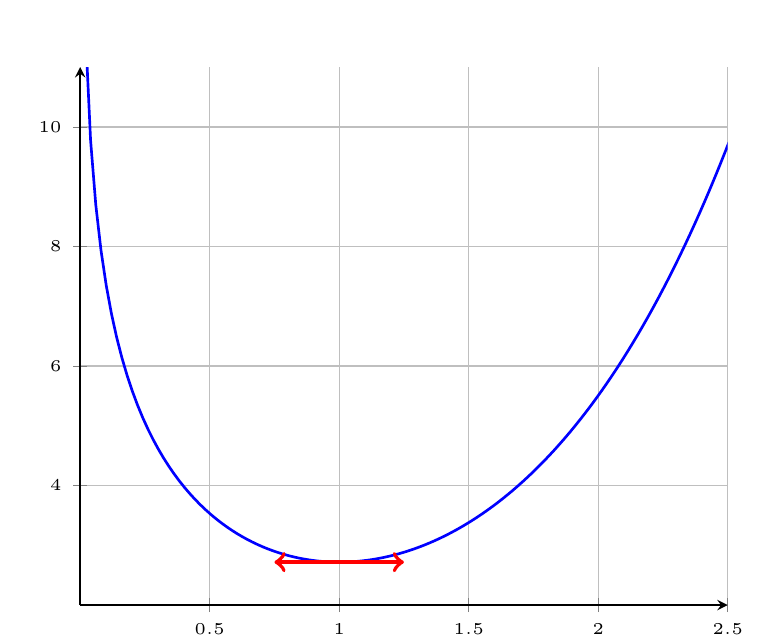
\begin{tikzpicture}[xscale=1.5, yscale = 1.5, scale =
        .8, % transform shape, %
        declare function = { %
          g(\x) = (exp(\x) - exp(1)*ln(\x); %
          h(\x) = exp(1); %
        },] %
        \pgfplotsset{every tick label/.append
          style={font=\tiny}} \begin{axis}[%
          xmin = 0, %
          xmax = 2.5, %
          ymin = 2, %
          ymax = 11, %
          no markers, %
          axis x line = center, %
          axis y line = center, %
          grid = both, %
          % xticklabels={},
          % ytick={-2,-1,0,1,2,3,4},%
          % yticklabels={-2,-1,0,1,2,3,4}%
          ] %
          \xdef\epsi{0.25}; %
          \addplot[samples=150, domain=0:3, blue, thick] {g(x)}; %
          \addplot[<->, samples=2, domain={1-\epsi}:{1+\epsi}, red,
          very thick]{h(x)}; %
        \end{axis}
      \end{tikzpicture}
    \end{center}
    
    
    %\newpage
    
    
    ~\\[-1.2cm]
  \end{proof}
    
    
  \item 
    \begin{noliste}{a)}
    \item Étudier les variations de la fonction $u:
    \begin{array}[t]{ccl}
      ]0,+\infty[ & \rightarrow & \R\\
      x & \mapsto & f'(x)-x
    \end{array}$
    
    \begin{proof}~
      \begin{noliste}{$\sbullet$}
      \item La fonction $f$ est deux fois dérivable sur $]0,+\infty[$
        donc $f'$ est dérivable sur $]0,+\infty[$.\\
        De plus, la fonction $x\mapsto x$ est dérivable sur
        $]0,+\infty[$. Ainsi, la fonction $u$ est dérivable sur
        $]0,+\infty[$ car elle est la différence de fonctions
        dérivables sur $]0,+\infty[$.
        
      \item Pour tout $x\in \ ]0,+\infty[$ : 
        \[
        u'(x) = f''(x) -1 = \ee^x +\dfrac{\ee}{x^2}-1 = \dfrac{x^2 \
          \ee^{x} + \ee - x^2}{x^2} = \dfrac{x^2 \ ( \ee^{x} - 1) +
          \ee}{x^2}
        \]
        Comme $x^2 > 0$, la quantité $u'(x)$ est du signe de $x^2 \ (
        \ee^{x} - 1) + \ee$.\\[.1cm]
        Or, comme $x > 0$, alors $\ee^x > \ee^0 = 1$. Comme de plus
        $x^2 > 0$ et $\ee > 0$, on en déduit : $u'(x) > 0$.
%         \[
%         \begin{array}{rcl@{\quad}>{\it}R{5cm}}
%           x>0 & \mbox{ donc } & \ee^x >\ee^0 = 1 & (car la fonction 
%           $\exp$ est strictement croissante sur $\R$)
%           \nl
%           \nl[-.4cm]
%           & \mbox{ d'où } & \ee^x -1>0
%           \\[.2cm]
%           & \mbox{ alors } & \ee^x -1 +\dfrac{\ee}{x^2}>0 & (car 
%           $\dfrac{\ee}{x^2}>0$)
%           \nl
%           \nl[-.4cm]
%           & \mbox{ ainsi } & u'(x)>0
%         \end{array}
%         \]
        \conc{La fonction $u$ est donc strictement croissante sur
          $]0,+\infty[$.}~
        
      \item On a : $\dlim{x\to 0} f'(x)=-\infty$ et $\dlim{x
          \to 0} x=0$.\\[.2cm]
        Donc $\dlim{x\to 0} u(x)=-\infty$.
        
      \item Déterminons alors la limite de $f$ en $+\infty$. Pour tout
        $x\in \ ]0,+\infty[$ :
        \[
        u(x)=\ee^x-\dfrac{\ee}{x}-x = \ee^x\left(1-\dfrac{\ee}{x\ee^x} - 
          \dfrac{x}{\ee^x}\right)
        \]
        Par croissances comparées, $\dlim{x\to+\infty} \dfrac{x}{\ee^x} = 
        0$. De plus $\dlim{x\to+\infty} \dfrac{\ee}{x\ee^x}=0$ et 
        $\dlim{x\to+\infty} \ee^x=+\infty$.\\[.2cm]
        Donc $\dlim{x\to +\infty} u(x)=+\infty$.
      \end{noliste}
      
      On obtient le tableau de variations suivant :
      
      \begin{center}
        \begin{tikzpicture}[scale=0.8, transform shape]
          \tkzTabInit[lgt=4,espcl=3] %
          { %
            $x$ /1, %
            Signe de $u'(x)$ /1, %
            Variations de $u$ /2
          } %
          {$0$, $+\infty$} %
          \tkzTabLine{ d, + , } % 
          \tkzTabVar{D-/$-\infty$, +/$+\infty$} %
        \end{tikzpicture}
      \end{center}~\\[-1.2cm]
%       ~\\[-1.2cm]
    \end{proof}
    

    %\newpage

	
  \item En déduire que l'équation $f'(x)=x$, d'inconnue $x\in \
    ]0,+\infty[$, admet une solution et une seule, notée $\alpha$, et
    montrer : $1<\alpha<2$.
  \end{noliste}      
 
    \begin{proof}~
      \begin{noliste}{$\sbullet$}
      \item On commence par remarquer :
        \[
        f'(x)=x \ \Leftrightarrow \ f'(x)-x=0 \ \Leftrightarrow \ u(x)=0
        \]
        On cherche donc à montrer que l'équation $u(x)=0$ admet une unique 
        solution sur $]0,+\infty[$.
        
    \item La fonction $u$ est :
      \begin{noliste}{$\stimes$}
      \item continue sur $]0,+\infty[$ (car dérivable sur $]0,+\infty[$ 
        d'après la question \itbf{4.a)}),
      \item strictement croissante sur $]0,+\infty[$.
      \end{noliste}
      Ainsi la fonction $u$ réalise une bijection de $]0,+\infty[$ sur
      $u(]0,+\infty|)$.
      \[
      u(]0,+\infty[)= \left] \dlim{x\to 0} u(x), \dlim{x\to +\infty}
        u(x)\right[ = \ ]-\infty, +\infty[
      \]
      Or $0\in \ ]-\infty,+\infty[$, donc l'équation $u(x)=0$ admet
      une unique solution $\alpha$ sur $]0,+\infty[$.%
      \conc{On en déduit que l'équation $f'(x)=x$ admet une unique
        solution $\alpha$ sur $]0,+\infty[$.}~
      
    \item Tout d'abord :
      \begin{noliste}{$\stimes$}
      \item $u(\alpha)=0$
      \item $u(1)=f'(1)-1=0-1=-1<0$
      \item $u(2)=f'(2)-2=\ee^2-\dfrac{\ee}{2}-2 > 0$\\[.1cm]
        En effet, d'après les encadrements donnés par l'énoncé, on
        obtient :
        \begin{noliste}{$-$}
        \item $7,3<\ee^2<7,4$, donc $5,3<\ee^2-2<5,4$
        \item $2,7<\ee<2,8$, donc $1,35 < \dfrac{\ee}{2} < 1,4$, d'où
          $-1,4<-\dfrac{\ee}{2}<-1,35$
        \end{noliste}
        Donc $3,9<\ee^2-2-\dfrac{\ee}{2}<4,05$, d'où $u(2)> 3,9>0$.
      \end{noliste}
      On en déduit : 
      \[
      u(1) < u(\alpha) < u(2)
      \]
      Or, d'après le théorème de la bijection, la bijection réciproque
      $u^{-1}: \ ]-\infty,+\infty[ \ \to \ ]0,+\infty[$ est
      strictement croissante. 
    \end{noliste}
    \conc{En appliquant $u^{-1}$ de part et d'autre de l'inégalité, on
      obtient : $1 < \alpha < 2$.}~\\[-1.1cm]
  \end{proof}
\end{noliste}


%\newpage


\subsection*{Partie II : Étude d'une suite, étude d'une série}
\noindent
On considère la suite réelle $(u_n)_{n\in\N}$ définie par :
\[
\left\{
  \begin{array}{l}
    u_0=2\\
    \forall n \in\N, \ u_{n+1}=f(u_n)
  \end{array}
\right.
\]
\begin{noliste}{1.}
  \setlength{\itemsep}{2mm}
  \setcounter{enumi}{4}
\item Montrer que, pour tout $n$ de $\N$, $u_n$ existe et $u_n\geq 2$.
  
  \begin{proof}~\\
    Démontrons par récurrence que : $\forall n\in\N$, $\PP{n}$, \quad
    où \quad $\PP{n}$ : $u_n$ existe et $u_n\geq 2$.
    \begin{noliste}{\fitem}
    \item {\bf Initialisation} : \\
      $u_0=2$. Donc $u_0\geq 2$.\\
      D'où $\PP{0}$.
      
    \item {\bf Hérédité} : soit $n\in\N$.\\
      Supposons $\PP{n}$ et démontrons $\PP{n+1}$ (c'est-à-dire
      $u_{n+1}$ existe et $u_{n+1}\geq 2$).\\
      Par hypothèse de récurrence, $u_n$ existe et $u_n\geq 2$.
      \begin{noliste}{$\sbullet$}
      \item La fonction $f$ est définie sur $]0,+\infty[$.\\
        Or $u_n \geq 2$, donc $u_n \in \ ]0,+\infty[$. Ainsi $u_{n+1}
        = f(u_n)$ existe.
        
      \item D'après la question \itbf{2.}, $\ee$ est le minimum de $f$ 
        sur $]0,+\infty|$, c'est-à-dire : 
        \[
        \forall x \in \ ]0,+\infty[, \ f(x) \geq \ee
        \]
        En appliquant cette inégalité à $x = u_n\in \ ]0,+\infty[$, on
        obtient :
        \[
        u_{n+1} \geq \ee > 2
        \]
      \end{noliste}
      D'où $\PP{n+1}$.
    \end{noliste}
    \conc{Par principe de récurrence, pour tout $n\in\N$, $u_n$ existe
      et $u_n\geq 2$.} ~\\[-1.2cm]
  \end{proof}
  
\item 
  \begin{noliste}{a)}
  \item Étudier les variations, puis le signe, de la fonction $g:
    \begin{array}[t]{ccl}
      [2,+\infty[ & \rightarrow & \R\\
      x& \mapsto & f(x)-x
    \end{array}$
    
    \begin{proof}~
      \begin{noliste}{$\sbullet$}
      \item La fonction $f$ est dérivable sur $[2,+\infty[$ d'après la
        question \itbf{1.a)}, et la fonction $x\mapsto x$ l'est aussi
        en tant que fonction polynomiale. La fonction $g$ est donc
        dérivable sur $[2,+\infty[$ en tant que différence de
        fonctions dérivables sur $[2,+\infty[$.
        
      \item Pour tout $x\in[2,+\infty[$, $g'(x)=f'(x)-1$.\\
        D'après la question \itbf{1.b)}, la fonction $f'$ est croissante. 
        Donc, pour tout $x\geq 2$ :
        \[
        f'(x)\geq f'(2)=\ee^2-\dfrac{\ee}{2} \geq 7,3-1,4=5,9>1
        \]
        On en déduit que pour tout $x\geq 2$, $g'(x)>0$.\\
        On obtient le tableau de variations suivant :\\[-.2cm]
  	\begin{center}
          \begin{tikzpicture}[scale=0.8, transform shape]
            \tkzTabInit[lgt=4,espcl=3] 
            {$x$ /1, Signe de $g'(x)$ /1, Variations de $g$ /2} 
            {$2$, $+\infty$}%
            \tkzTabLine{ , + , } 
            \tkzTabVar{-/ $g(2)$, +/$+\infty$}
          \end{tikzpicture}
        \end{center}
        

        %\newpage

      
      \item Déterminons maintenant le signe de $g$. Comme $g$ est
        croissante sur $[2, +\infty[$, on a :
        \[
        \forall x\geq 2, \ g(x) \geq g(2)
        \] 
        Il ssufit alors de démontrer : $g(2) > 0$ pour pouvoir
        conclure. Calculons : 
        \[
        g(2) = f(2)-2 = \ee^2 - \ee\ln(2) - 2
        \]
        D'après les approximations de l'énoncé :
        \begin{noliste}{$\stimes$}
	\item $7,3 < \ee^2 < 7,4$
	\item $2,7 < \ee < 2,8$ et $0,6 < \ln(2) < 0,7$, donc :
          \[
          1,62=2,7\times 0,6 < \ee \ln(2) < 2,8\times 0,7=1,96
          \]
          D'où $-1,96<-\ee\ln(2) <-1,62$.
        \end{noliste}
        Ainsi : $\ee^2 -\ee\ln(2)-2 > 7,3-1,96-2 = 3,34 > 0$.\\
        On en déduit : $g(2)>0$.%
        \conc{$\forall x\in [2,+\infty[$, $g(x)>0$}~\\[-1.4cm]
      \end{noliste}
    \end{proof}
    
  \item En déduire que la suite $(u_n)_{n\in\N}$ est croissante.
	
    \begin{proof}~\\
      Soit $n \in \N$.
      \begin{noliste}{$\sbullet$}
      \item D'après la question \itbf{6.a)} : $\forall x \geq 2$,
        $g(x)>0$. Autrement dit, pour tout $x \geq 2$ :
        \[
        f(x) > x
        \]
      \item En appliquant cette inégalité à $x = u_n \geq 2$ (question
        \itbf{5.}), on obtient : 
        \[
        u_{n+1} = f(u_n) > u_n
        \]
      \end{noliste}
      \conc{Ainsi, pour tout $n\in\N$, $u_{n+1} > u_n$. La suite
        $(u_n)$ est donc (strictement) croissante.}~\\[-1.2cm]
    \end{proof}
  \end{noliste}
  
  
\item Démontrer que la suite $(u_n)_{n\in\N}$ admet $+\infty$ pour 
  limite.
  
  \begin{proof}~\\
    On sait que la suite $(u_n)$ est croissante (question
    \itbf{6.b)}), donc :
    \begin{noliste}{$-$}
    \item soit $(u_n)$ est de plus majorée, et alors elle converge.
    \item soit $(u_n)$ n'est pas majorée, et alors elle diverge vers 
      $+\infty$.
    \end{noliste}
    Supposons par l'absurde que $(u_n)$ est majorée.
    \begin{noliste}{$\sbullet$}
    \item Dans ce cas, la suite $(u_n)$ est croissante et majorée donc
      elle converge vers un réel $\ell$.\\
      D'après la question \itbf{5.}, on a : $\forall n\in\N$, $u_n
      \geq 2$.\\
      Par passage à la limite dans cette inégalité, on obtient : $\ell
      \geq 2$.
      
    \item D'autre part, par définition : $\forall n\in\N$,
      $u_{n+1}=f(u_n)$.\\
      Par passage à la limite ($f$ est continue sur $[2,+\infty[$), on
      obtient : $\ell = f(\ell)$, donc $g(\ell)=0$.\\
      Ceci est absurde car, d'après la question \itbf{6.a)} : $\forall
      x\geq 2$, $g(x)>0$, donc $\forall x\geq 2$, $g(x)\neq 0$.
    \end{noliste}
    \conc{Ainsi, la suite $(u_n)$ n'est pas majorée et elle diverge
      vers $+\infty$}


    %\newpage


    ~\\[-1.4cm]
  \end{proof}

\item Écrire un programme en \Scilab{} qui, étant donné un réel $A$,
  renvoie un entier naturel $N$ tel que $u_N\geq A$.

\begin{proof}~
\begin{scilab}
   & A = input(\ttq{}A=\ttq{}) \nl %
   & N = 0 \nl %
   & u = 2 \nl %
   & \tcFor{while} u < A \nl %
   & \qquad u = exp(u) - \%e \Sfois{} ln(u) \nl %
   & \qquad N = N + 1 \nl %
   & \tcFor{end} \nl %
   & disp(N) \nl %
\end{scilab}~\\[-.8cm]
\end{proof}


\item 
  \begin{noliste}{a)}
  \item Démontrer : $\forall x\in[2,+\infty[$, $2\ln(x)\leq x \leq
    \dfrac{\ee^x}{3}$.
    
    \begin{proof}~
      \begin{noliste}{$\sbullet$}
      \item Montrons que : $\forall x \in[2,+\infty[$, $2\ln(x)\leq x$.\\
        La fonction $h:x\mapsto \ln(x)$ est concave sur
        $[2,+\infty[$.\\
        Sa courbe représentative est donc située en dessous de ses
        tangentes.\\
        En particulier, elle est sous sa tangente au point $2$,
        c'est-à-dire :
        \[
        \forall x \in [2,+\infty[, \ h(x) \leq h'(2)(x-2) + h(2) =
        \dfrac{1}{2}(x-2) + \ln(2)
        \]
        Ainsi, pour tout $x\in[2,+\infty[$ :
        \[
        2 \ln(x) \ \leq \ (x-2) + 2\ln(2) = x + 2(\ln(2)-1) \leq x
        \]
        En effet, comme : $0,6<\ln(2)<0,7$, alors : $2(\ln(2)-1)<0$. %
        \conc{$\forall x \in [2,+\infty[$, $2\ln(x)\leq x$}
        
      \item Montrons que : $\forall x \in[2,+\infty[$, $x\leq
        \dfrac{\ee^x}{3}$.\\[.2cm]
        Considérons la fonction $h : x \mapsto \dfrac{\ee^x}{3} - x$.\\
        La fonction $h$ est dérivable sur $[2,+\infty[$ comme somme de
        fonctions dérivables sur $[2,+\infty[$.\\
        Soit $x\in[2,+\infty[$.
        \[
        h'(x)=\dfrac{\ee^x}{3}-1 = \dfrac{\ee^x-3}{3}
        \]
        Comme $3>0$, la quantité $h'(x)$ est du signe de $\ee^x-3$.\\
        Or, comme $x \geq 2$, par croissance de la fonction $\exp$ :
        \[
        \ee^x \ \geq \ \ee^2 > 7,3
        \]
        Et ainsi, $\ee^x - 3 > 4,3 > 0$ et donc $h'(x) > 0$.


        %\newpage


        \noindent
        On obtient le tableau de variations suivant :        

        \begin{center}
          \begin{tikzpicture}[scale=0.8, transform shape]
            \tkzTabInit[lgt=4,espcl=3] 
            {$x$ /1, Signe de $h'(x)$ /1, Variations de $h$ /2} 
            {$2$, $+\infty$}%
            \tkzTabLine{ ,+,  } 
            \tkzTabVar{-/$h(2)$, +/$+\infty$}
          \end{tikzpicture}
        \end{center}
        
        De plus $h(2)=\dfrac{\ee^2}{3}-2=\dfrac{\ee^2-6}{3}>0$ car
        $\ee^2>7,3$.\\
        Or $h$ est strictement croissante sur $[2,+\infty[$, donc pour
        tout $x\in[2,+\infty[$ : 
        \[
        h(x) \geq h(2) \geq 0
        \]
      \end{noliste}
      \conc{On en conclut : $\forall x\in[2,+\infty[$, $x \leq
        \dfrac{\ee^x}{3}$.}
      
      ~\\[-1.4cm]
    \end{proof}
    
  \item En déduire : $\forall n\in\N$, $u_{n+1} \geq
    \dfrac{6-\ee}{2}u_n$.
	
    \begin{proof}~\\
      Soit $n\in\N$. 
      \begin{noliste}{$\sbullet$}
      \item D'après la question précédente :
        \[
        \forall x\in[2,+\infty[, \ 2 \ln(x) \leq x \leq \dfrac{\ee^x}{3}
        \]
        En appliquant cette double inégalité à $x = u_n \in [2,
        +\infty$, on obtient :
        \[
        2\ln(u_n) \leq u_n \leq \dfrac{\ee^{u_n}}{3}
        \]

      \item Comme $2\ln(u_n) \leq u_n$, alors $-\ee \ln(u_n) \geq
        -\dfrac{\ee}{2}u_n$.
        
      \item Comme $u_n \leq \dfrac{\ee^{u_n}}{3}$, alors
        $\ee^{u_n}\geq 3u_n$.
      \end{noliste}
      On en déduit :
      \[
      u_{n+1} = f(u_n) = \ee^{u_n} - \ee \ln(u_n) \geq 3 u_n
      -\dfrac{\ee}{2} u_n = \dfrac{6-\ee}{2}u_n
      \]
      \conc{$\forall n\in\N$, $u_{n+1} \geq \dfrac{6-\ee}{2}u_n$}
    \end{proof}
    

    %\newpage
	

  \item Déterminer la nature de la série de terme général
    $\dfrac{1}{u_n}$.
	
    \begin{proof}~\\
      Soit $n\in\N$.
      \begin{noliste}{$\sbullet$}
      \item D'après la question \itbf{9.b)} :
        \[
        \begin{array}{rclllllllll}
          u_{n+1} & \geq & \dfrac{6-\ee}{2} & u_n
          \\[.4cm]
          & \geq & \dfrac{6-\ee}{2} & \dfrac{6-\ee}{2}
          &  u_{n-1} & & & &
          & = & \left(\dfrac{6-\ee}{2}\right)^2 u_{n-1}
          \\[.4cm]
          & \geq & \dfrac{6-\ee}{2} & \dfrac{6-\ee}{2} & 
          \dfrac{6-\ee}{2} & u_{n-2} & & &
          & = & \left(\dfrac{6-\ee}{2}\right)^3 u_{n-2}
          \\[.4cm]
          & \cdots & 
          \\[.2cm]
          & \geq & \dfrac{6-\ee}{2} & \dfrac{6-\ee}{2} &
          \dfrac{6-\ee}{2} & \dfrac{6-\ee}{2} & \cdots 
          & \dfrac{6-\ee}{2} & u_0 
          & = & \left(\dfrac{6-\ee}{2}\right)^{n+1} u_0
        \end{array}
        \]
        {\it On peut démontrer rigoureusement ce résultat par
          récurrence (voir remarque en page suivante).  }\\
        Comme $u_0=2$, on obtient : $\forall n\in\N$, $u_n \geq 2
        \left(\dfrac{6-\ee}{2}\right)^n$.
      \item Or, d'après la question \itbf{5.} : $\forall n\in\N$,
        $u_n\geq 2 >0$.\\
        On obtient donc, par passage à l'inverse :
        \[
        \forall n \in \N, \ \dfrac{1}{u_n} \leq \dfrac{1}{2}
        \left(\dfrac{2}{6-\ee}\right)^n
        \]
      \item On a alors :
        \begin{noliste}{$\stimes$}
        \item $\forall n \in \N$, $0\leq \dfrac{1}{u_n} \leq
          \left(\dfrac{2}{6-\ee}\right)^n$
        \item la série $\Sum{}{} \left(\dfrac{2}{6-\ee}\right)^n$ est
          une série géométrique de raison $\dfrac{2}{6-\ee}$ avec
          $\left\vert
            \dfrac{2}{6-\ee} \right\vert <1$.\\[.2cm]
          (en effet, $3<3,2<6-\ee<3,3<4$ donc
          $-1<\dfrac{2}{4}<\dfrac{2}{6-\ee}<\dfrac{2}{3}<1$)\\
          Elle est donc convergente.
        \end{noliste}
      \end{noliste}
    \conc{Par critère de comparaison de séries à termes positifs, la 
    série $\Sum{}{} \dfrac{1}{u_n}$ est convergente.}
  
  

  %\newpage


  ~\\[-1.4cm]
\end{proof}
\end{noliste}
\end{noliste}

\subsection*{Partie III : Étude d'intégrales généralisées}
\begin{noliste}{1.}
\setlength{\itemsep}{2mm}
\setcounter{enumi}{9}
\item Montrer que l'intégrale $\dint{0}{1} f(x)\dx$ converge et 
calculer 
cette intégrale.

\begin{proof}~
   \begin{noliste}{$\sbullet$}
    \item La fonction $f$ est continue sur $]0,1]$.
    \item Soit $a\in \ ]0,1]$.
    \[
     \begin{array}{rcl@{\quad}>{\it}R{4cm}}
      \dint{a}{1}f(x)\dx & = & \dint{a}{1} (\ee^x- \ee \ln(x)) \dx
      \\[.4cm]
      & = & \dint{a}{1}\ee^x\dx - \ee\dint{a}{1}\ln(x)\dx
      & (par linéarité de l'intégrale)
      \nl
      \nl[-.2cm]
      & = & \Prim{\ee^x}{a}{1} -\ee\Prim{x\ln(x)-x}{a}{1}
      \\[.4cm]
      & = & \ee-\ee^a -\ee \ (\bcancel{1\ln(1)}-1-(a\ln(a)-a))
      \\[.2cm]
      & = & 2\ee -\ee^a +\ee \ a \ln(a) -\ee \ a
      \\[.2cm]
      & \tendd{a}{0} & 2\ee -1
     \end{array}
    \]
    En effet, $\dlim{a\to0}\ee^a=1$, $\dlim{a\to0}\ee \ a =0$ et 
    $\dlim{a\to0} a\ln(a)=0$ par croissances comparées.
   \end{noliste}
   \conc{Ainsi, l'intégrale impropre $\dint{0}{1}f(x)\dx$ converge et
     $\dint{0}{1}f(x)\dx = 2\ee-1$.}


   %\newpage


   ~\\[-1.2cm]
 \end{proof}
 
\item L'intégrale $\dint{1}{+\infty} f(x)\dx$ converge-t-elle ?

  \begin{proof}~\\
    On a les informations suivantes :
    \begin{noliste}{$\stimes$}
    \item $f(x)=\ee^x - \ee\ln(x) \eqx{+\infty} \ee^x$.
    \item $\forall x \in[1,+\infty[$, $\ee^x\geq 0$\\
      D'après la question \itbf{2.} : $\forall x\in[1,+\infty[$,
      $f(x)\geq 0$.
    \item L'intégrale $\dint{1}{+\infty} \ee^x\dx$ diverge.
    \end{noliste}
    Par critère d'équivalence des intégrales généralisées de fonctions
    continues positives, l'intégrale impropre
    $\dint{1}{+\infty}f(x)\dx$ est divergente.~\\[-.4cm] %
    \conc{L'intégrale $\dint{1}{+\infty} f(x)\dx$ diverge.}~\\[-1cm]
    ~\\[-1.4cm]
\end{proof}

%\newpage

\item Montrer que l'intégrale $\dint{2}{+\infty} \dfrac{1}{f(x)}\dx$
  converge.  On pourra utiliser le résultat de la question
  \itbf{9.a)}.

\begin{proof}~
\begin{noliste}{$\sbullet$}
\item Soit $x\in[2,+\infty[$.\\
D'après la question \itbf{9.a)}, $2\ln(x)\leq x$. Donc :
\[
f(x)=\ee^x - \ee \ln(x)\geq \ee^x - \ee \, \frac{x}{2}.
\]
Donc, par décroissance de la fonction inverse sur $\R_+^*$, 
$\dfrac{1}{f(x)}\leq \dfrac{1}{\ee^x-\ee \, \frac{x}{2}}$.
Or :
\[
\ee^x - \ee\frac{x}{2} = \ee^x \left(1 - 
\frac{\ee}{2} \, \frac{x}{\ee^x}\right) \eqx{+\infty} \ee^x
\]
car $\dlim{x\to +\infty} \dfrac{x}{\ee^x}=0$ par croissances comparées. 
Donc
$\dfrac{1}{\ee^x-\ee \, \frac{x}{2}} \eqx{+\infty} \ee^{-x}$.\\[.2cm]
Et comme 
$\ee^{-x}= \oox{+\infty}\left(\dfrac{1}{x^2}\right)$, alors
$\dfrac{1}{\ee^x-\ee \, \frac{x}{2}} = \oox{+\infty} 
\left(\dfrac{1}{x^2}\right)$.

\item On sait donc :
\begin{noliste}{$\stimes$}
  \item $\dfrac{1}{\ee^x-\ee \, \frac{x}{2}} = \oox{+\infty} 
  \left(\dfrac{1}{x^2}\right)$
  
  \item $\forall x\in [2,+\infty[$, $\dfrac{1}{\ee^x-\ee \, \frac{x}{2}}
  \geq 0$
  
  \item L'intégrale $\dint{2}{+\infty} \dfrac{1}{x^2}\dx$ est une 
  intégrale de Riemann impropre en $+\infty$ d'exposant strictement 
  supérieur à $1$. Elle est donc convergente.
\end{noliste}
Par critère de négligeabilité d'intégrales généralisées de fonctions
continues positives, l'intégrale impropre $\dint{2}{+\infty}
\dfrac{1}{\ee^x-\ee \frac{x}{2}} \dx$ converge.

\item On sait alors :
\begin{noliste}{$\stimes$}
  \item $\forall x\in [2,+\infty[$, $0\leq \dfrac{1}{f(x)}\leq 
  \dfrac{1}{\ee^x-\ee \, \frac{x}{2}}$.
  \item D'après la question \itbf{2.} : $\forall x\in 
  [2,+\infty[$, $f(x)\neq 0$.\\[.2cm]
  Donc la fonction $x\mapsto \dfrac{1}{f(x)}$ est continue sur 
  $[2,+\infty[$ en tant qu'inverse d'une fonction continue
  sur $[2,+\infty[$ qui ne 
  s'annule pas.
  \item L'intégrale $\dint{2}{+\infty} 
  \dfrac{1}{\ee^x-\ee \frac{x}{2}} \dx$ converge.
  \end{noliste}

\conc{Par critère de comparaison d'intégrales généralisées de fonctions 
 continues positives,\\ 
 l'intégrale $\dint{2}{+\infty} 
 \dfrac{1}{f(x)}\dx$ converge.}~\\[-1.4cm]
\end{noliste}
\end{proof}
\end{noliste}

%\newpage

\subsection*{Partie IV : Étude d'une fonction de deux variables
  réelles}

\noindent
On considère la fonction $F: \ ]1,+\infty[^2 \rightarrow \R$, de classe 
$\Cont 2$ sur l'ouvert $]1,+\infty[^2$, définie, pour tout $(x,y)$ de 
$]1,+\infty[^2$, par :
\[
F(x,y)=f(x)+f(y)-xy.
\]
\begin{noliste}{1.}
\setlength{\itemsep}{2mm}
\setcounter{enumi}{12}
\item Montrer que $F$ admet un point critique et un seul et qu'il 
s'agit 
de $(\alpha,\alpha)$, le réel $\alpha$ ayant été défini à la question 
{\bf 4.} de la partie {\bf I}.

\begin{proof}~
\begin{noliste}{$\sbullet$}
\item La fonction $F$ est de classe $\Cont{2}$ sur $]1,+\infty[^2$, 
donc, a fortiori, de classe $\Cont{1}$ sur $]1,+\infty[^2$.

\item Soit $(x,y)\in \ ]1,+\infty[^2$.
\[
\partial_1(F)(x,y)=f'(x)-y \ \mbox{ et } \ \partial_2(F)(x,y)=f'(y)-x
\]

\item Donc $(x,y)$ est un point critique de $F$ si et seulement si :
\[
\begin{array}{rcl@{\quad}>{\it}R{5cm}}
\nabla(F)(x,y)=\begin{smatrix}
0\\0
\end{smatrix} 
&
\Leftrightarrow 
&
\left\{
\begin{array}{l}
\partial_1(F)(x,y)=0
\\[.2cm]
\partial_2(F)(x,y)=0
\end{array}
\right. 
\
\Leftrightarrow
\
\left\{
\begin{array}{l}
f'(x)-y=0
\\[.2cm]
f'(y)-x=0
\end{array}
\right. 
\\[.8cm]
&
\Leftrightarrow 
&
\left\{
\begin{array}{l}
y=f'(x)
\\[.2cm]
x=f'(y)
\end{array}
\right. 
\
\Leftrightarrow 
\
\left\{
\begin{array}{l}
xy=xf'(x)
\\[.2cm]
xy=yf'(y)
\end{array}
\right.
&
(car $x>0$ et $y>0$)
\nl
\nl[-.2cm]
& 
\Leftrightarrow 
&
\left\{
\begin{array}{l}
xy=xf'(x)
\\[.2cm]
xf'(x)=yf'(y)
\end{array}
\right.
\
\Leftrightarrow
\
\left\{
\begin{array}{l}
 y = f'(x)
 \\[.2cm]
 xf'(x) = yf'(y)
\end{array}
\right.
\quad (*)
\end{array}
\]
\item On introduit la fonction $v:x\mapsto xf'(x)$. Montrons qu'elle
est injective.\\
Soit $x \in \ ]1,+\infty[$.
\[
 v(x) = xf'(x) = x \left(\ee^x - \dfrac{\ee}{x}\right) = 
 x\ee^x - \ee
\]
La fonction $v$ est dérivable sur $]1,+\infty[$ en tant que somme et
produit de fonctions dérivables sur l'intervalle
$]1,+\infty[$.
\[
 \forall x\in \ ]1,+\infty[, \quad v'(x) = \ee^x + x\ee^x = (x+1) \ee^x
 >0
\]
Donc la 
fonction $v$ 
est strictement croissante.\\
En particulier, la fonction $v$ est injective.
 
\item Reprenons alors le système $(*)$. Par injectivité de $v$ :
\[
\left\{
\begin{array}{l}
y=f'(x)
\\[.2cm]
v(x)=v(y)
\end{array}
\right. 
\
\Leftrightarrow 
\
\left\{
\begin{array}{l}
y=f'(x)
\\[.2cm]
x=y
\end{array}
\right. 
\
\Leftrightarrow 
\
\left\{
\begin{array}{l}
x=f'(x)
\\[.2cm]
x=y
\end{array}
\right. 
\
\Leftrightarrow 
\
\left\{
\begin{array}{l}
x=\alpha
\\[.2cm]
x=y
\end{array}
\right.
\]
En effet, d'après la question \itbf{4.b)}, l'équation $x=f'(x)$
admet le réel $\alpha$ comme unique solution sur
l'intervalle $]1,+\infty[$.\\
On obtient alors :
\[
\nabla(F)(x,y)=\begin{smatrix}
0\\0
\end{smatrix} 
\
\Leftrightarrow 
\
\left\{
\begin{array}{l}
x=\alpha
\\[.2cm]
x=y
\end{array}
\right.
\
\Leftrightarrow 
\
\left\{
\begin{array}{l}
x=\alpha
\\[.2cm]
y=\alpha
\end{array}
\right.
\]
\conc{La fonction $F$ admet un point critique et un seul et il s'agit 
de $(\alpha,\alpha)$.}~\\[-1.2cm]
\end{noliste}
\end{proof}

%\newpage

\item \begin{noliste}{a)}
	\item Déterminer la matrice hessienne de $F$ en 
	$(\alpha,\alpha)$.
	
	\begin{proof}~
	\begin{noliste}{$\sbullet$}
	\item La fonction $F$ est de classe $\Cont{2}$ sur 
	$]1,+\infty[^2$. 
	\item Soit $(x,y)\in \ ]1,+\infty[^2$.
	\[
	\nabla^2(F)(x,y)=\begin{smatrix}
	\partial_{1,1}^2(F)(x,y) & \partial_{1,2}^2(F)(x,y)
	\\[.2cm]
	\partial_{2,1}^2(F)(x,y) & \partial_{2,2}^2(F)(x,y)
	\end{smatrix}
	=
	\begin{smatrix}
	 f''(x) & -1
	 \\[.2cm]
	 -1 & f''(y)
	\end{smatrix}
	\]
	\conc{Donc $\nabla^2(F)(\alpha,\alpha)=\begin{smatrix}
	f''(\alpha) & -1\\
	-1 & f''(\alpha)
	\end{smatrix}$.}~\\[-1.4cm]
	\end{noliste}
	\end{proof}
	
	\item La fonction $F$ admet-elle un extremum local en 
	$(\alpha,\alpha)$ ? Si oui, s'agit-il d'un maximum local ou 
	s'agit-il d'un minimum local ?
	
	\begin{proof}~\\
          Déterminons les valeurs propres de
          $\nabla^2(F)(\alpha,\alpha)$.\\[.1cm]
          On cherche donc les valeurs de $\lambda$ pour lesquelles
          $\nabla^2(F)(\alpha,\alpha) - \lambda \, I_2$ n'est pas
          inversible, c'est-à-dire pour lesquelles
          $\det(\nabla^2(F)(\alpha,\alpha)-\lambda \, I_2)=0$\\[.1cm]
          Soit $\lambda\in\R$.
	\[
	\det(\nabla^2(F)(\alpha,\alpha)-\lambda \, I_2)
	=
	\det \left( 
	\begin{matrix}
	f''(\alpha)-\lambda & -1
	\\[.2cm] 
	-1 & f''(\alpha)-\lambda
	\end{matrix}
	\right)
	= 
	(f''(\alpha)-\lambda)^2-1
	=(f''(\alpha)-\lambda-1)(f''(\alpha)-\lambda+1)
	\]
	Donc les valeurs propres de $\nabla^2(F)(\alpha,\alpha)$ sont
	$f''(\alpha)-1$ et $f''(\alpha)+1$.\\[.2cm]
	Or pour tout $x\in \ ]0,+\infty[$,
        $f''(x)=\ee^x+\dfrac{\ee}{x^2}> \ee^x \geq 1$. Donc
        $f''(\alpha)-1>0$ et $f''(\alpha)+1>0$.%
        \conc{Ainsi $F$ admet un minimum local en
          $(\alpha,\alpha)$.}~\\[-1cm]
	\end{proof}
	\end{noliste}
\end{noliste}


%\newpage


\section*{Exercice 2}

\noindent
On note $E = \R_2[X]$ l'espace vectoriel des polynômes de degré
inférieur ou égal à $2$ et $\B = (1,X,X^2)$ la base canonique de $E$.
Pour tout polynôme $P$ de $E$, on note indifféremment $P$ ou $P(X)$.\\
Pour tout $(\alpha,\beta,\gamma)\in\R^3$, la dérivée $P'$ du polynôme
$P=\alpha+\beta X+\gamma X^2$ est le polynôme $P' = \beta+2\gamma X$,
et la dérivée seconde $P''$ de $P$ est le polynôme $P'' = 2\gamma$.\\
On note, pour tout polynôme $P$ de $E$ :
\[
a(P) = P-XP', \quad b(P) = P-P', \quad c(P) = 2XP-(X^2-1) \ P'
\]
Par exemple : $a(X^2) = X^2-X(2X) = -X^2$.\\
Enfin, on note $f = b\circ a - a \circ b$.




\subsection*{Partie I : Étude de $a$}

\begin{noliste}{1.}
  \setlength{\itemsep}{2mm}
\item Montrer que $a$ est un endomorphisme de $E$.
  
  \begin{proof}~
    \begin{noliste}{$\sbullet$}
    \item Montrons que $a$ est une application linéaire.\\
      Soit $(P_1,P_2)\in E^2$ et $(\lambda_1,\lambda_2)\in\R^2$.
      \[
      \begin{array}{rcl}
        \big(a(\lambda_1 \cdot P_1+ \lambda_2 \cdot P_2)\big)(X) & =
        & \big(\lambda_1 \cdot P_1+\lambda_2 \cdot P_2\big)(X) -
        X \ \big(\lambda_1 \cdot P_1+\lambda_2 \cdot P_2 \big)'(X)
        \\[.2cm]
        & = & \lambda_1 \cdot P_1(X) + \lambda_2 \cdot P_2(X)
        -X \ \big(\lambda_1 \cdot P_1'(X) + \lambda_2 \cdot P_2'(X)\big)
        \\[.2cm] 
        & = & \lambda_1 \cdot P_1(X)+\lambda_2 \cdot P_2(X)-\lambda_1 \cdot 
        XP_1'(X) - \lambda_2 \cdot X 
        P_2'(X)
        \\[.2cm]
        & = & \lambda_1 \cdot (P_1(X)-XP_1'(X))+\lambda_2 \cdot(P_2(X)-XP_2'(X))
        \\[.2cm]
        & = & \lambda_1 \cdot (a(P_1))(X)+ \lambda_2 \cdot (a(P_2))(X)
        \\[.2cm]
        & = & \big(\lambda_1 \cdot a(P_1)+ \lambda_2 \cdot a(P_2) \big)(X)
      \end{array}
      \]
      Et ainsi : $a(\lambda_1 \cdot P_1+ \lambda_2 \cdot P_2) =
      \lambda_1 \cdot a(P_1)+ \lambda_2 \cdot a(P_2)$.
      
    \item Montrons que $a(E)\subset E$. Autrement dit, montrons que
      pour
      tout $P\in E$, $a(P)\in E$.\\
      Soit $P\in E$. Alors il existe $(\alpha,\beta,\gamma)\in\R^3$
      tels que $P(X)=\alpha+\beta X+\gamma X^2$. Donc :
      \[
      \begin{array}{rcl}
        (a(P))(X) & = & P(X)-XP'(X)
        \\[.2cm]
        & = & \alpha +\beta X+\gamma X^2 -X(\beta +2\gamma X)
        \\[.2cm]
        & = & -\gamma X^2 + \alpha
      \end{array}
      \]
      Ainsi, $a(P)$ est un polynôme de degré inférieur ou égal à $2$ :
      $a(P)\in E$.
    \end{noliste}
    \conc{On en déduit que $a$ est un endomorphisme de $E$.}~\\[-1.2cm]
  \end{proof}


%\newpage


\item
  \begin{noliste}{a)}
  \item Montrer que la matrice $A$ de $a$ dans la base $\B$ de $E$ est
    $A = 
    \begin{smatrix} 
      1 & 0 & 0 \\ 
      0 & 0 & 0 \\ 
      0 & 0 & -1
    \end{smatrix}$.
    
    \begin{proof}~\\
      Pour éviter les confusions, on notera $\B = (P_0,P_1,P_2)$ la
      base canonique de $\R_2[X]$ :
      \[
      P_0(X)=1, \quad P_1(X)=X, \quad P_2(X)=X^2
      \]
      \begin{noliste}{$\sbullet$}
      \item $\big( a(P_0) \big)(X) = P_0(X) - X \times P_0'(X)= 1 - 0
        = 1 = P_0(X)$. On en déduit :
        \[
        a(P_0) = 1 \cdot P_0 + 0 \cdot P_1 + 0 \cdot P_2
        \]
        Et ainsi : $\Mat_{\B}(a(P_0)) =
	\begin{smatrix}
          1\\
          0\\
          0
	\end{smatrix}$.
	
      \item $\big( a(P_1) \big) = P_1(X) - X\times P_1'(X) = X - X =
        0$. On en déduit :
        \[
        a(P_1) = 0 \cdot P_0 + 0 \cdot P_1 + 0 \cdot P_2
        \]
        Ainsi : $\Mat_{\B}(a(P_1)) =
	\begin{smatrix}
          0\\
          0\\
          0
	\end{smatrix}$.
	
      \item $\big( a(P_2) \big)(X) = P_2(X) - X \times P_2'(X) = X^2 -
        2 X^2 = -X^2 = -P_2(X)$. On en déduit : 
        \[
        a(P_2) = 0 \cdot P_0 + 0\cdot P_1 - 1 \cdot P_2
        \]
	Ainsi : $\Mat_{\B}(a(P_2)) =
	\begin{smatrix}
          0\\
          0\\
          -1
	\end{smatrix}$.
      \end{noliste}      
      \conc{On en conclut : $A = \Mat_\B(a) =
        \begin{smatrix} 
          1 & 0 & 0 \\
          0 & 0 & 0 \\
          0 & 0 & -1
	\end{smatrix}$.}~\\[-1.2cm]
    \end{proof}
    
  \item Déterminer le rang de la matrice $A$.
    
    \begin{proof}~
      \[
      \rg(A)=\rg \left(
        \begin{smatrix}
	  1 & 0 & 0\\
	  0 & 0 & 0\\
	  0 & 0 & -1
        \end{smatrix}
      \right)
      \begin{arrayEg}
        C_2 \leftrightarrow C_3
      \end{arrayEg}
      \rg\left(
        \begin{smatrix}
	  1 & 0 & 0\\
	  0 & 0 & 0\\
	  0 & -1 & 0
        \end{smatrix}
      \right)
      \begin{arrayEg}
        L_2 \leftrightarrow L_3
      \end{arrayEg}
      \rg\left(
        \begin{smatrix}
	  1 & 0 & 0\\
	  0 & -1 & 0\\
	  0 & 0 & 0
        \end{smatrix}
      \right)
      =2
      \]
      \conc{$\rg(A)=2$}~\\[-1.2cm]
    \end{proof}
  \end{noliste}
  
\item L'endomorphisme $a$ est-il bijectif ? Déterminer $\kr(a)$ et
  $\im(a)$.

  \begin{proof}~
    \begin{noliste}{$\sbullet$}
    \item Tout d'abord : $\dim(\im(a))=\rg(A)=2\neq 3 = \dim (E)$.\\
      Donc $\im(A)\neq E$. Ainsi l'endomorphisme $a$ n'est pas
      surjectif.%
      \conc{On en déduit que l'endomorphisme $a$ n'est pas bijectif.}

    \item D'après le théorème du rang :
      \[
      \begin{array}{ccccc}
        \dim(E) & = & \dim(\kr(a)) & + & \rg(a)
        \\
        \shortparallel & & & & \shortparallel
        \\
        3 & & & & 2
      \end{array}
      \]
      D'où : $\dim(\kr(a))=1$.
      

      %\newpage


      \noindent
      D'après la question précédente : $a(P_1) = 0$. Ainsi $P_1 \in
      \kr(a)$. \\
      La famille $(P_1)$ est une famille libre, car elle est
      constituée d'un polynôme non nul.\\
      Comme $\Card( (P_1) ) = 1 = \dim(\kr(a))$, on en déduit que
      $(P_1)$ est une base de $\kr(a)$.\\[-.2cm] %
      \conc{$\kr(a) = \Vect{P_1}$}~\\[-.6cm]
      
    \item Par caractérisation de l'image d'une application linéaire :
      \[
      \im(a) =\Vect{a(P_0), \ a(P_1), \ a(P_2)} = \Vect{P_0, \ 0, \ -P_2}
      = \Vect{P_0, \ P_2}
      \]
      Ainsi :
      \begin{noliste}{$\stimes$}
      \item la famille $(P_0,P_2)$ engendre $\im(a)$.
      \item $\Card\big( (P_0,P_2) \big) = 2 = \dim\big( \im(a) \big)$.
      \end{noliste}
      La famille $(P_0,P_2)$ est donc une base de $\im(a)$. %
      \conc{$\im(a) = \Vect{P_0,P_2}$}% = \Vect{1,X^2}$}
    \end{noliste}
    
    ~\\[-1.2cm]
  \end{proof}
  On admet, pour la suite de l'exercice, que $b$ et $c$ sont des
  endomorphismes de $E$.\\
  On note $B$ et $C$ les matrices, dans la base $\B$ de $E$, de $b$ et
  $c$ respectivement.
\end{noliste}


%\newpage


\subsection*{Partie II : Étude de $b$}

\begin{noliste}{1.}
  \setlength{\itemsep}{2mm} %
  \setcounter{enumi}{3}
\item Montrer que $b$ est bijectif et que, pour tout $Q$ de $E$, on a
  : $b^{-1}(Q) = Q + Q' + Q''$.

  \begin{proof}~
    \begin{noliste}{$\sbullet$}
    \item Notons $g : E \to E$ l'endomorphisme de $E$ qui à tout $Q
      \in E$ associe $g(Q) = Q + Q' + Q''$.\\
      Il s'agit de démontrer que $b$ est bijective, de réciproque
      $g$. Pour ce faire, on démontre :
      \[
      b \circ g = \id_E \qquad \text{ et } \qquad g \circ b = \id_E
      \]

    \item Soit $P \in E$.
      \[
      \begin{array}{rcl@{\quad}>{\it}R{5cm}}
        (b \circ g)(P) & = & b \big( g(P) \big)
        \\[.2cm]
        & = & b(P+P'+P'')
        \\[.2cm]
        & = & b(P)+b(P')+b(P'') & (par linéarité de $b$)
        \nl
        \nl[-.2cm]
        & = & (P-\bcancel{P'})+(\bcancel{P'}-\bcancel{P''})+(\bcancel{P''}-P''')
        \\[.2cm]
        & = & P-P''' 
        \\%[.2cm]
        & = & P & ($P'''=0$ car $P$ est un polynôme de degré au plus $2$)
      \end{array}
      \]
      On en déduit : $b \circ g = \id_E$.\\%[.1cm]
      De même :
      \[
      \begin{array}{rcl}
        (g \circ b) (P) & = & g\big( P-P' \big) 
        \\[.2cm]
        & = & (P-P') + (P-P')' + (P-P')'' 
        \\[.2cm]
        & = & P - P' + P' - P'' + P'' - P''' \ = \ P - P''' \ = \ P
      \end{array}
      \]
    \end{noliste}
    \concL{Les applications $g$ et $b$ sont bijectives et réciproques
      l'une de l'autre. \\[.1cm]
      On en déduit notamment : $\forall Q \in E$, $b^{-1}(Q) = g(Q) =
      Q + Q' + Q''$.}{13.4}%~\\[-1cm]
    ~\\[-1.4cm]
  \end{proof}


  %\newpage


\item 
  \begin{noliste}{a)}
  \item Montrer que $b$ admet une valeur propre et une seule et
    déterminer celle-ci.
	
    \begin{proof}~
      \begin{noliste}{$\sbullet$}
      \item Comme $B$ est la matrice représentative de $b$ dans la
        base $\B$ :
        \[
        \spc(b) \ = \ \spc(B)
        \]
        On commence donc par déterminer cette matrice $B$.
        \begin{noliste}{$\stimes$}
	\item $\big( b(P_0) \big) (X) = P_0(X) - P_0'(X) = 1 =
          P_0(X)$. On en déduit :
          \[
          b(P_0) = 1 \cdot P_0 + 0 \cdot P_1 + 0 \cdot P_2
          \]
          Et ainsi : $\Mat_{\B}(b(P_0)) =
          \begin{smatrix}
            1\\
            0\\
            0
          \end{smatrix}$.
	
	\item $\big( b(P_1) \big) (X) = P_1(X) - P_1'(X) = X - 1 =
          -P_0(X) + P_1(X)$. On en déduit :
          \[
          b(P_1) = -1 \cdot P_0 + 1 \cdot P_1 + 0 \cdot P_2
          \]
          Et ainsi : $\Mat_{\B}(b(P_1)) =
          \begin{smatrix}
            -1\\
            1\\
            0
          \end{smatrix}$.

	\item $\big( b(P_2) \big) (X) = P_2(X) - P_2'(X) = X^2 - 2X =
          -2 \ P_1(X) + P_2(X)$. On en déduit :
          \[
          b(P_1) = 0 \cdot P_0 - 2 \cdot P_1 + 1 \cdot P_2
          \]
          Et ainsi : $\Mat_{\B}(b(P_2)) =
          \begin{smatrix}
            0\\
            -2\\
            1
          \end{smatrix}$.
	\end{noliste}
	\conc{On en déduit : $B = \Mat_\B(b) = 
          \begin{smatrix} 
            1 & -1 & 0 \\
            0 & 1 & -2\\ 
            0 & 0 & 1
          \end{smatrix}
          $.}

      \item La matrice $B$ est triangulaire supérieure.\\
        Ses valeurs propres sont donc ses coefficients diagonaux et
        $\spc(B) = \{ 1 \}$.%
        % Ainsi $\spc(B)=\{1\}$.\\
        % De plus $B$ est la matrice représentative de $b$ dans la
        % base $\B$, donc $\spc(b)=\spc(B)$.%
	\conc{On en déduit : $\spc(b) = \spc(B) = \{1\}$.}~\\[-1cm]
      \end{noliste}
    \end{proof}
    
  \item L'endomorphisme $b$ est-il diagonalisable ?
    
    \begin{proof}~\\
      Montrons par l'absurde que $b$ n'est pas diagonalisable.\\
      Supposons que $b$ est diagonalisable, alors $B = \Mat_{B}(b)$
      l'est aussi.\\
      Il existe donc une matrice inversible $P \in \M{3}$ et une
      matrice diagonale $D \in \M{3}$ dont les coefficients diagonaux
      sont les valeurs propres de $B$ telles que $B = PDP^{-1}$.\\
      Or $1$ est la seule valeur propre de $B$. Ainsi $D = I$ et :
      \[
      B = PDP^{-1} = PIP^{-1} = PP^{-1} = I
      \]
      Absurde !%
      \conc{On en déduit que $b$ n'est pas diagonalisable.}
      ~\\[-1.4cm]
    \end{proof}
  \end{noliste}
\end{noliste}

\subsection*{Partie III : Étude de $c$}

\begin{noliste}{1.}
\setlength{\itemsep}{2mm}
\setcounter{enumi}{5}
\item Montrer : $C=\begin{smatrix}
0 & 1 & 0\\ 
2 & 0 & 2\\ 
0 & 1 & 0
\end{smatrix}$.

\begin{proof}~
\begin{noliste}{$\sbullet$}
\item $(c(P_0))(X)=2X\times P_0(X)-(X^2-1)\times P_0'(X)=2X=0\cdot 
P_0(X)+2\cdot P_1(X)+0\cdot P_2(X)$\\[.2cm]
Ainsi : $\Mat_{\B}(c(P_0)) =
	\begin{smatrix}
	 0\\
	 2\\
	 0
	\end{smatrix}$.

\item $(c(P_1))(X)=2X\times P_1(X) - (X^2-1)\times P_1'(X) 
=X^2+1=1\cdot P_0(X)+0\cdot 
P_1(X)+1\cdot P_2(X)$\\[.2cm]
Ainsi : $\Mat_{\B}(c(P_1)) =
	\begin{smatrix}
	 1\\
	 0\\
	 1
	\end{smatrix}$.
	
\item $(c(P_2))(X)=2X\times P_2(X) - (X^2-1)\times P_2'(X)=2X=0\cdot 
P_0(X)+2\cdot P_1(X)+0\cdot P_2(X)$\\[.2cm]
Ainsi : $\Mat_{\B}(c(P_2)) =
	\begin{smatrix}
	 0\\
	 2\\
	 0
	\end{smatrix}$.
\end{noliste}

\conc{On en déduit : $C=\Mat_\B(c)=\begin{smatrix}
    0 & 1 & 0\\ 
    2 & 0 & 2\\ 
    0 & 1 & 0
  \end{smatrix}$.}~\\[-1cm]
\end{proof}

\item L'endomorphisme $c$ est-il bijectif ?

  \begin{proof}~
    \[
    \rg(c) \ = \ \rg(C) \ = \
    \rg\left(
      \begin{smatrix}
        0 & 1 & 0\\
        2 & 0 & 2\\
        0 & 1 & 0
      \end{smatrix}
    \right)
    \begin{arrayEg}
      L_3\leftarrow L_3-L_1
    \end{arrayEg}
    \rg\left(
      \begin{smatrix}
        0 & 1 & 0\\
        2 & 0 & 2\\
        0 & 0 & 0
      \end{smatrix}
    \right)
    \ = \ 2
    \]
    On en déduit $\dim(\im(c)) = \rg(c) = 2\neq 3 = \dim(E)$. \\
    Donc : $\im(c)\neq E$, ce qui implique que l'endomorphisme 
    $c$ n'est pas surjectif.%
    \conc{Ainsi l'endomorphisme $c$ n'est pas bijectif.}~\\[-1cm]
  \end{proof}


%\newpage


\item 
  \begin{noliste}{a)}
  \item Déterminer une matrice $R$, carrée d'ordre trois, inversible,
    dont les coefficients de la première ligne sont tous égaux à $1$,
    et une matrice $D$, carrée d'ordre trois, diagonale, à
    coefficients diagonaux dans l'ordre croissant, telles que $C =
    RDR^{-1}$.
    
    \begin{proof}~
      \begin{noliste}{$\sbullet$}
      \item Déterminons les valeurs propres de $C$.\\
	Soit $\lambda \in \R$.\\
	On cherche les réels $\lambda$ tels que la matrice $C-\lambda
        I_3$ n'est
	pas inversible, c'est-à-dire tels que $\rg(C-\lambda I_3)<3$.\\
	\[
	\begin{array}{rcl}
          \rg(C-\lambda \, I_3) & = & \rg\left( 
            \begin{smatrix}
              -\lambda & 1 & 0\\
              2 & -\lambda & 2\\
              0 & 1 & -\lambda
            \end{smatrix}
          \right)
          \\[.8cm]
          &
          \begin{arrayEg}
            L_1 \leftrightarrow L_2
          \end{arrayEg}
          &
          \rg\left(
            \begin{smatrix}
              2 & -\lambda & 2\\
              -\lambda & 1 & 0\\
              0 & 1 & -\lambda
            \end{smatrix}
          \right)
          \\[.8cm]
          &
          \begin{arrayEg}
            L_2 \leftarrow 2L_2 +\lambda L_1
          \end{arrayEg}
          &
          \rg\left(
            \begin{smatrix}
              2 & -\lambda & 2\\
              0 & 2-\lambda^2 & 2\lambda\\
              0 & 1 & -\lambda
            \end{smatrix}
          \right)
          \\[.8cm]
          &
          \begin{arrayEg}
            L_2 \leftrightarrow L_3
          \end{arrayEg}
          &
          \rg\left(
            \begin{smatrix}
              2 & -\lambda & 2\\
              0 & 1 & -\lambda\\
              0 & 2-\lambda^2 & 2\lambda
            \end{smatrix}
          \right)
          \\[.8cm]
          &
          \begin{arrayEg}
            L_3 \leftarrow L_3 - (2-\lambda^2)L_2
          \end{arrayEg}
          &
          \rg\left(
            \begin{smatrix}
              2 & -\lambda & 2\\
              0 & 1 & -\lambda\\
              0 & 0 & q(\lambda)
            \end{smatrix}
          \right)
	\end{array}
	\]
	où $q(\lambda)=2\lambda + \lambda(2-\lambda^2) =
        \lambda(2+(2-\lambda^2)) = \lambda(4-\lambda^2) =
        \lambda(2-\lambda)(2+\lambda)
	$.\\
	La réduite obtenue est triangulaire supérieure.\\
	Elle est non inversible ssi l'un de ses coefficients diagonaux
        est nul. Ainsi :
	\[
	\rg(C-\lambda \, I_3)<3 \ \Leftrightarrow \ q(\lambda)=0 \
        \Leftrightarrow \ \lambda \in \{0,2,-2\}
	\]
	\conc{Ainsi : $\spc(C)=\{-2,0,2\}$.}
	
      \item Déterminons $E_0(C)$, le sous-espace propre de $C$ 
	associé à la valeur propre $0$.\\
	Soit $X=
	\begin{smatrix}
          x\\
          y\\
          z
	\end{smatrix} \in \M{3,1}$.	
	\[
	\begin{array}{rcl}
          X\in E_0(C) & \Leftrightarrow & CX = 0_{\M{3,1}}
          \\[.2cm]
          & \Leftrightarrow & 
          \begin{smatrix}
            0 & 1 & 0\\
            2 & 0 & 2\\
            0 & 1 & 0
          \end{smatrix}
          \begin{smatrix}
            x\\
            y\\
            z
          \end{smatrix}
          =
          \begin{smatrix}
            0\\
            0\\
            0
          \end{smatrix}
          \\[.6cm]
          & \Leftrightarrow & \left\{
            \begin{array}{rrrrrcl}
              & & y & & & = & 0\\
              2x & & & + & 2z &= & 0\\
              & & y & & & = & 0
            \end{array}
          \right.
          \\[.8cm]
          & \Leftrightarrow & \left\{
            \begin{array}{rcr}
              y & = & 0\\
              x & = & -z
            \end{array}
          \right.
	\end{array}
	\]
	

	%\newpage


	\noindent
	On obtient alors :
	\[
	\begin{array}{rcl}
          E_0(C) & = & \{
          \begin{smatrix}
            x\\
            y\\
            z
          \end{smatrix}
          \in \M{3,1} \ 
          \vert \
          y=0 \mbox{ et } x=-z \}
          \\[.6cm]
          & = & \{
          \begin{smatrix}
            -z\\
            0\\
            z
          \end{smatrix}
          \ | \ z\in\R
          \}
          \ = \ \{z \cdot
          \begin{smatrix}
            -1\\
            0\\
            1
          \end{smatrix}
          \ | \ z\in\R
          \}
          \\[.6cm]
          & = & \Vect{
            \begin{smatrix}
              -1\\
              0\\
              1
            \end{smatrix}
          }
          \ = \ \Vect{
            \begin{smatrix}
              1\\
              0\\
              -1
            \end{smatrix}
          }
	\end{array}
	\]
	
      \item Déterminons $E_2(C)$, le sous-espace propre de $C$
	associé à la valeur propre $2$.\\
	Soit $X=
	\begin{smatrix}
          x\\
          y\\
          z
	\end{smatrix} \in \M{3,1}$	
	\[
	\begin{array}{rcl}
          X\in E_2(C) & \Longleftrightarrow & (C-2 \, 
          I_3) \ X = 0_{\M{3,1}}
          \\[.2cm]
          & \Longleftrightarrow &
          \begin{smatrix}
            -2 & 1 & 0\\
            2 & -2 & 2\\
            0 & 1 & -2
          \end{smatrix}
          \begin{smatrix}
            x\\
            y\\
            z
          \end{smatrix}
          =
          \begin{smatrix}
            0\\
            0\\
            0
          \end{smatrix}
          \\[.6cm]
          & \Longleftrightarrow & 
          \left\{
            \begin{array}{rrrrrcl}
              -2x & + & y & & & = & 0\\
              2x & - & 2y & + & 2z & = & 0\\
              & & y &- & 2z & = & 0
            \end{array}
          \right.
          \\[.8cm]
          &
          \begin{arrayEq}
            L_2 \leftarrow L_2+L_1
          \end{arrayEq}
          &
          \left\{
            \begin{array}{rrrrrcl}
              -2x&+ & y & & & = & 0\\
              &- &y & + & 2z &= & 0\\
              & & y &- & 2z& = & 0
            \end{array}
          \right.
          \\[.8cm]
          &
          \begin{arrayEq}
            L_3 \leftarrow L_3 + L_2
          \end{arrayEq}
          &
          \left\{
            \begin{array}{rrrcr}
              -2x & + & y & = & 0\\
              & & y & = & 2z
            \end{array}
          \right.
          \\[.8cm]
          &
          \begin{arrayEq}
            L_1 \leftarrow L_1 - L_2
          \end{arrayEq}
          &
          \left\{
            \begin{array}{rrrcr}
              -2x & & & = & -2z\\
              & & y & = & 2z
            \end{array}
          \right.
          \\[.8cm]
          & \Longleftrightarrow & 
          \left\{
            \begin{array}{rcr}
              x & = & z\\
              y & = & 2z
            \end{array}
          \right.
	\end{array}
	\]	
	On obtient alors :
	\[
	\begin{array}{rcl}
          E_2(C) & = & \{
          \begin{smatrix}
            x\\
            y\\
            z
          \end{smatrix}
          \in \M{3,1}
          \ | \ 
          x=z \mbox{ et } y=2z \}
          \\[.6cm]
          & = & \{
          \begin{smatrix}
            z\\
            2z\\
            z
          \end{smatrix}
          \ | \ 
          z \in\R \}
          \ = \ \{z \cdot
          \begin{smatrix}
            1\\
            2\\
            1
          \end{smatrix}
          \ | \ 
          z \in\R \}
          \\[.6cm]
          & = & \Vect{
            \begin{smatrix}
              1\\
              2\\
              1
            \end{smatrix}
          }
        \end{array}
	\]
	
        
	%\newpage
        
	
      \item Déterminons $E_{-2}(C)$, le sous-espace propre de $C$
	associé à la valeur propre $-2$.\\
	Soit $X =
	\begin{smatrix}
          x\\
          y\\
          z
	\end{smatrix} \in \M{3,1}$	
	\[
	\begin{array}{rcl}
          X\in E_{-2}(C) &\Longleftrightarrow & (C+2\, 
          I_3)X=0_{\M{3}}
          \\[.6cm]
          & \Longleftrightarrow & 
          \begin{smatrix}
            2 & 1 & 0\\
            2 & 2 & 2\\
            0 & 1 & 2
          \end{smatrix}
          \begin{smatrix}
            x\\
            y\\
            z
          \end{smatrix}
          =
          \begin{smatrix}
            0\\
            0\\
            0
          \end{smatrix}
          \\[.6cm]
          & \Longleftrightarrow & 
          \left\{
            \begin{array}{rrrrrcl}
              2x & + & y & & & = & 0\\
              2x & + & 2y & + & 2z & = & 0\\
              & & y & + & 2z & = & 0
            \end{array}
          \right.
          \\[.8cm]
          &
          \begin{arrayEq}
            L_2 \leftarrow L_2 - L_1
          \end{arrayEq}
          &
          \left\{
            \begin{array}{rrrrrcl}
              2x & + & y & & & = & 0\\
              & & y & + & 2z & = & 0\\
              & & y & + & 2z & = & 0
            \end{array}
          \right.
          \\[.8cm]
          &
          \begin{arrayEq}
            L_3 \leftarrow L_3 - L_2
          \end{arrayEq}
          &
          \left\{
            \begin{array}{rrrcr}
              2x & + & y & = & 0\\
              & & y & = & -2z
            \end{array}
          \right.
          \\[.8cm]
          &
          \begin{arrayEq}
            L_1 \leftarrow L_1 - L_2
          \end{arrayEq}
          &
          \left\{
            \begin{array}{rrrcr}
              2x & & & = & 2z\\
              & & y & = & -2z
            \end{array}
          \right.
          \\[.8cm]
          & \Longleftrightarrow & 
          \left\{
            \begin{array}{rcr}
              x & = & z\\
              y & = & -2z
            \end{array}
          \right.
	\end{array}
	\]	
	On obtient alors :
	\[
	\begin{array}{rcl}
          E_{-2}(C) & = & \{ 
          \begin{smatrix}
            x\\
            y\\
            z
          \end{smatrix}
          \in \M{3,1}
          \ | \ x=z \mbox{ et } y=-2z
          \}
          \\[.6cm]
          & = & \{ 
          \begin{smatrix} 
            z\\
            -2z\\
            z
          \end{smatrix}
          \ | \ z\in\R
          \}
          \ = \ \{ z \cdot
          \begin{smatrix}
            1\\
            -2\\
            1
          \end{smatrix}
          \ | \ z\in\R
          \}
          \\[.6cm]
          & = & \Vect{
            \begin{smatrix}
              1\\
              -2\\
              1
            \end{smatrix}
          }
	\end{array}
	\]
	
      \item En résumé :
	\begin{noliste}{$\stimes$}
        \item $C\in\M{3}$
        \item $C$ admet $3$ valeurs propres {\bf distinctes} : $-2$,
          $0$, $2$.
	\end{noliste}
	On en déduit que la matrice $C$ est diagonalisable.\\
	Il existe donc une matrice $R\in\M{3}$ inversible ($R$ est la
        concaténation des vecteurs bases des sous-espaces propres de
        $C$), et $D\in\M{3}$ diagonale, dont les coefficients
        diagonaux sont les valeurs propres de $C$, telles que
        $C=RDR^{-1}$.%
	\conc{En posant $D = 
          \begin{smatrix}
            -2 & 0 & 0\\
            0 & 0 & 0\\
            0 & 0 & 2
          \end{smatrix}$ et $R=\begin{smatrix}
            1 & 1 & 1\\ 
            -2 & 0 & 2\\
            1 & -1 & 1
          \end{smatrix}$, on obtient bien : $C=RDR^{-1}$.}~\\[-1.2cm]
      \end{noliste}
    \end{proof}
    

    %\newpage

	
  \item En déduire que l'endomorphisme $c$ est diagonalisable et
    déterminer une base de $E$ constituée de vecteurs propres de
    $c$.
    
    \begin{proof}~
      \begin{noliste}{$\sbullet$}
      \item D'après la question \itbf{8.a)}, la matrice $C$ est
        diagonalisable.\\
        Or c'est une matrice représentative de $c$ dans
        la base $\B$.%~\\[-.6cm]
        \conc{On en déduit que l'endomorphisme $c$ est
          diagonalisable.}  %

      \item Une base de $E$ constituée de vecteurs propres est alors
        la concaténation des bases des sous-espaces propres de $c$ que
        l'on a déterminés à la question précédente.\\
        De plus :
        \[
        \begin{smatrix}
          1\\
          0\\
          -1
        \end{smatrix}
        = \Mat_{\B}(1 \cdot P_0+ 0\cdot P_1-1 \cdot P_2),
        \]
        \[
        \begin{smatrix}
          1\\
          2\\
          1
        \end{smatrix}
        = \Mat_{\B}(1 \cdot P_0+2 \cdot P_1+1\cdot P_2),
        \]~\\[-.8cm]
        \[
        \begin{smatrix}
          1\\
          -2\\
          1
        \end{smatrix}
        = \Mat_{\B}(1\cdot P_0-2\cdot P_1+1 \cdot P_2)
        \]
        Donc :
        \[
        E_0(c)=\Vect{P_0-P_2}, \qquad E_{2}(c)=\Vect{P_0+2P_1+P_2},
        \qquad E_{-2}(c)=\Vect{P_0-2P_1+P_2}
        \]~\\[-1.4cm]
      
        \conc{Une base de $E$ constituée de vecteurs propres de $c$
          est
          alors \\[.1cm]
          $(P_0 - 2 \cdot P_1 + P_2, P_0 - P_2, P_0 + 2 \cdot P_1 +
          P_2)$.}~\\[-.8cm]
      \end{noliste}
    \end{proof}
  \end{noliste}
\end{noliste}


\subsection*{Partie IV : Étude de $f$}
\begin{noliste}{1.}
\setlength{\itemsep}{2mm}
\setcounter{enumi}{8}
\item Montrer : $\forall P\in E$, $f(P)=P'$.

  \begin{proof}~\\
    Soit $P\in E$.
    \[
    \begin{array}{rcl}
      (f(P))(X) & = & (b\circ a(P))(X) -(a \circ b(P))(X)
      \\[.2cm]
      & = & b(P(X)-XP'(X)) -a(P(X)-P'(X))
      \\[.2cm]
      & = & (P(X) - XP'(X))-(P(X) - XP'(X))' - \Big((P(X) - P'(X)) -
      X \ (P(X) - P'(X))'\Big) 
      \\[.2cm]
      & = & 
      \bcancel{P(X)}-XP'(X) - \Big(\bcancel{P'(X)} - (\bcancel{P'(X)}+XP''(X))
      \Big)
      \\[.2cm]
      & & - \ \Big(\bcancel{P(X)}-P'(X)-XP'(X)+XP''(X)\Big)
      \\[.2cm]
      & = & 
      -\bcancel{XP'(X)}+\bcancel{XP''(X)}+P'(X)+\bcancel{XP'(X)}-\bcancel{
        XP''(X) }
      \\[.2cm]
      & = & P'(X)
    \end{array}
    \]~\\[-1.2cm]
    \conc{Pour tout $P\in E$, $f(P)=P'$.}~\\[-1cm]
  \end{proof}


%\newpage 


\item En déduire : $(BA-AB)^3=0$.

  \begin{proof}~\\
    Soit $P\in E$.\\
    Tout d'abord, d'après la question \itbf{9} : $f(P)=P'$.\\[.1cm]
    De plus, comme $P$ est un polynôme de degré au plus $2$, on en
    déduit : $(f\circ f \circ f)(P) =P'''=0$.\\
    Ceci étant vrai pour tout $P\in E$, on en déduit : $f\circ f \circ
    f = 0_{\LL{E}}$.

    en passant à l'écriture matricielle :
    \[
    \Mat_\B(f\circ f \circ f)= \Mat_\B(0_{\LL{E}})= 0_{\M{3}}
    \]
    Or $\Mat_\B(f\circ f \circ f)= \Mat_{\B}(f^3)
    =\left(\Mat_\B(f)\right)^3=(\Mat_\B(b\circ a -a \circ
    b))^3=(BA-AB)^3$.%
    \conc{Ainsi : $(BA-AB)^3=0$.}~\\[-1cm]
  \end{proof}
\end{noliste}



%\newpage

\section*{Exercice 3}

\noindent
On considère une urne contenant initialement une boule bleue et deux
boules rouges.\\
On effectue, dans cette urne, des tirages successifs de la façon
suivante : on pioche une boule au hasard et on note sa couleur, puis
on la replace dans l'urne en ajoutant une boule de la même couleur que
celle qui vient d'être obtenue.\\[.1cm]
Pour tout $k$ de $\N^*$, on note :
\begin{tabular}[t]{R{12cm}}
  $B_k$ l'événement : \og on obtient une boule bleue au $\eme{k}$ tirage \fg{}, 
  \nl
  \nl[-.3cm]
  $R_k$ l'événement : \og on obtient une boule rouge au $\eme{k}$
  tirage \fg{}.
\end{tabular}

\subsection*{Partie I : Simulation informatique}

\begin{noliste}{1.}
\item Recopier et compléter la fonction suivante afin qu'elle simule
  l'expérience étudiée et renvoie le nombre de boules rouges obtenues
  lors des $n$ premiers tirages, l'entier $n$ étant entré en argument.
  \begin{scilab}
    & \tcFun{function} \tcVar{s} = EML(\tcVar{n}) \nl %
    & \qquad b = 1 \commentaire{b désigne le nombre de boules bleues
      présentes dans l'urne} \nl %
    & \qquad r = 2 \commentaire{r désigne le nombre de boules rouges
      présentes dans l'urne} \nl %
    & \qquad \tcVar{s} = 0 \commentaire{s désigne le nombre de boules 
    rouges obtenues lors des n tirages} \nl %
    & \qquad \tcFor{for} k = 1:\tcVar{n} \nl %
    & \qquad \qquad x = rand() \nl %
    & \qquad \qquad \tcIf{if} ... \tcIf{then} \nl %
    & \qquad \qquad \qquad  ... \nl %
    & \qquad \qquad \tcIf{else} \nl %
    & \qquad \qquad \qquad  ... \nl %
    & \qquad \qquad \tcIf{end} \nl %
    & \qquad \tcFor{end} \nl %
    & \tcFun{endfunction}
  \end{scilab}

  \begin{proof}~
    \begin{noliste}{$\sbullet$}
    \item Le programme consiste, au fur et à mesure des tirages :
      \begin{noliste}{$\stimes$}
      \item à mettre à jour les variables {\tt b} et {\tt r},
        désignant respectivement le nombre de boules bleues et le
        nombre de boules rouges présentes dans l'urne.
      \item à comptabiliser le nombre {\tt s} de boules rouges tirées.
      \end{noliste}

    \item L'instruction {\tt rand()} permet de simuler une \var de loi
      uniforme sur $]0,1[$.\\
      Le résultat obtenu (stocké dans la variable {\tt x}) va
      permettre de simuler le tirage :
      \begin{noliste}{$\stimes$}
      \item si $\mt{x} \in \ ]0, \frac{\mt{b}}{\mt{b+r}}[$, on
        considère qu'on a tiré une boule bleue dans l'urne. Dans ce
        cas :
        \begin{noliste}{}
        \item on ajoute une boule bleue dans l'urne : {\tt b = b+1}.
        \item on ne modifie pas le nombre de boules rouges de l'urne.
        \item on ne modifie pas le nombre de boules rouges tirées.
        \end{noliste}
        {\it ($\frac{\mt{b}}{\mt{b+r}}$ est la proportion de boules
          bleues dans l'urne)}

      \item si $\mt{x} \in [\frac{\mt{b}}{\mt{b+r}}, 1[$, on considère
        qu'on a tiré une boule rouge dans l'urne. Dans ce cas :
        \begin{noliste}{}
        \item on ajoute une boule rouge dans l'urne : {\tt r = r+1}.
        \item on ne modifie pas le nombre de boules bleues de l'urne.
        \item on met à jour le nombre de boules rouges tirées : {\tt s
            = s+1}.
        \end{noliste}
        {\it ($1 - \frac{\mt{b}}{\mt{b+r}} = \frac{\mt{r}}{\mt{b+r}}$
          est la proportion de boules rouges dans l'urne)}
      \end{noliste}
    \end{noliste}


    %\newpage


    \noindent
    En résumé, on obtient :\\[-.6cm]
    \begin{scilabC}{6}
      & \tcIf{if} x < b / (b+r) \tcIf{then} \nl %
      & \qquad b = b + 1 \nl %
      & \tcIf{else} \nl %
      & \qquad r = r + 1 \nl %
      & \qquad \tcVar{s} = \tcVar{s} + 1 \nl %
      & \tcIf{end} \nl %
    \end{scilabC}~\\[-1cm]
%     \begin{scilab}
%       & function s = EML(n) \nl %
%       & \qquad b = 1 \commentaire{b désigne le nombre de boules 	
%	bleues
%         présentes dans l'urne} \nl %
%       & \qquad r = 2 \commentaire{r désigne le nombre de boules 	
%	rouges
%         présentes dans l'urne} \nl %
%       & \qquad s = 0 \commentaire{s désigne le nombre de boules 	
%	rouges
%         obtenues lors des n tirages} \nl %
%       & \qquad for k = 1:n \nl %
%       & \qquad \qquad s = rand() \nl %
%       & \qquad \qquad if x < b / (b+r) then \nl %
%       & \qquad \qquad \qquad b = b + 1 \nl %
%       & \qquad \qquad else \nl %
%       & \qquad \qquad \qquad r = r + 1 \nl %
%       & \qquad \qquad \qquad s = s + 1 \nl %
%       & \qquad \qquad end \nl %
%       & \qquad end \nl %
%       & endfunction
%     \end{scilab}        
    ~\\[-1.4cm]
  \end{proof}

\item On exécute le programme suivant :
  \begin{scilab}
    & n = 10 \nl %
    & m = 0 \nl %
    & \tcFor{for} i = 1:1000 \nl % 
    & \qquad m = m + EML(n) \nl %
    & \tcFor{end} \nl %
    & disp(m/1000)
  \end{scilab}
  On obtient $6.657$. Comment interpréter ce résultat ?
  
  \begin{proof}~
    \begin{noliste}{$\sbullet$}
    \item La fonction {\tt EML} permet de simuler la \var $S_n$
      (introduite plus tard dans l'énoncé) égale au nombre de boules
      rouges obtenues au cours des $n$ premiers tirages.

    \item Le programme consiste à simuler (à l'aide de l'appel {\tt
        EML(10)}) de simuler un grand nombre de fois ($N = 1000$ est
      ce grand nombre) la \var $S_{10}$.\\
      Formellement, on souhaite obtenir un $N$-uplet $(v_1, \ldots,
      v_{N})$ qui correspond à l'observation d'un $N$-échantillon
      $(V_1, \ldots, V_{N})$ de la \var $S_{10}$.\\
      {\it (cela signifie que les \var $V_1$, \ldots, $V_{N}$ sont
        indépendantes et sont de même loi que $S_{10}$)}

    \item La variable {\tt m}, initialisée à $0$, est mise à jour à
      chaque tour de boucle $i$ par l'ajout de la dernière valeur
      $v_i$ créée. De sorte que, à l'issue de la boucle, la variable
      {\tt m} contient : $\Sum{i=1}{N} v_i$.

    \item Enfin, en ligne \ligne{6}, l'instruction {\tt disp(m/1000)}
      permet de réaliser l'affichage de la division par $1000$ de la
      valeur contenue dans {\tt m}. C'est donc la valeur :
      $\dfrac{1}{N} \ \Sum{i=1}{N} v_i$ qui est affichée.\\
      Il s'agit de la moyenne empirique des $N$ simulations de la \var
      $S_{10}$.

    \item Or, en vertu de la loi faible des grands nombres (LfGN) :
        \[
        \mbox{moyenne de l'observation} = \dfrac{1}{N} \ \Sum{i =
          1}{N} v_i \ \simeq \ \E(S_{10})
        \]

%       successivement $X_1$, $X_2$, \ldots, $X_{1000}$, qui sont $1000$
%       variables indépendantes, et de même loi que la \var
%       $S_{10}$.\\
%       Autrement dit, $(X_1, X_2, \ldots, X_{1000})$ est un
%       $1000$-échantillon de la \var $S_{10}$.
%     \item Le programme renvoie une simulation de $\overline{X_{1000}}
%       = \dfrac{X_1 + \ldots + X_{1000}}{1000}$, \var donnant la
%       moyenne empirique associée à \var $S_{10}$. En vertu de la loi
%       faible des grands nombres, la \var $\overline{X_{1000}}$
%       converge en probabilité vers la variable aléatoire constante
%       égale à $\E(S_{10})$.
    \end{noliste}
    \concL{Le programme fournit une approximation de $\E(S_{10})$. Le
      résultat obtenu : $\E(S_{10}) \simeq 6.657$ signifie qu'on
      obtient en moyenne un peu moins de $7$ boules rouges lorsque
      l'on procède à $10$ tirages successifs (en respectant le
      protocole de l'énoncé) dans l'urne.}{15.4}


    %\newpage


    ~\\[-1.4cm]
  \end{proof}
\end{noliste}

\subsection*{Partie II : Rang d'apparition de la première boule bleue 
et rang d'apparition de la première boule rouge}

\noindent 
On définit la variable aléatoire $Y$ égale au rang d'apparition de la
première boule bleue et la variable aléatoire $Z$ égale au rang
d'apparition de la première boule rouge.

\begin{noliste}{1.}
  \setcounter{enumi}{2}
\item
  \begin{noliste}{a)}
  \item Montrer que : \ $\forall n \in \N^*, \ \Prob(\Ev{Y = n}) =
    \dfrac{2}{(n+1)(n+2)}$.

    \begin{proof}~\\
      Soit $n \in \N^*$.
      \begin{noliste}{$\sbullet$}
      \item Si $n \geq 2$, $\Ev{Y = n} = R_1 \cap \ldots \cap 
      R_{n-1} \cap B_n$.\\
        D'après la formule des probabilités composées :
        \[
        \begin{array}{cccccccccccc}
          & \multicolumn{11}{l}{\Prob(\Ev{Y = n})} \\[.2cm]
          = & \multicolumn{11}{l}{\Prob(R_1 \cap \ldots \cap R_{n-1}
            \cap B_n)} \\[.2cm] 
          = & \Prob(R_1) & \times & \Prob_{R_1}(R_2) & \times & 
	  \Prob_{R_1
            \cap R_2}(R_3) & \times & \ldots & \times & \Prob_{R_1 \cap 
	    \ldots
            \cap R_{n-2}}(R_{n-1}) & \times & \Prob_{R_1 \cap \ldots 
	    \cap
            R_{n-1}}(B_n) \\[.2cm]
          = & \dfrac{2}{\bcancel{3}} & \times &
          \dfrac{\bcancel{3}}{\bcancel{4}} & \times & 
          \dfrac{\bcancel{4}}{\bcancel{5}} & \times & \ldots &
          \times & \dfrac{\bcancel{n}}{n+1} & \times &
          \dfrac{1}{n+2} \\[.4cm]
          = & \multicolumn{11}{l}{\dfrac{2}{(n+1)(n+2)}}
        \end{array}         
        \]

      \item On a utilisé dans l'écriture précédente, pour tout $k
        \in \llb 2, n-1 \rrb$, l'égalité :
        \[
        \Prob_{R_1 \cap \ldots \cap R_{k-1}}(R_k) = \dfrac{k+1}{k+2}
        \]
        En effet, si l'événement $R_1 \cap \ldots \cap R_{k-1}$ est
        réalisé c'est qu'on a tiré une boule rouge lors de chacun des
        $k-1$ premiers tirages. Juste avant le $\eme{k}$ tirage,
        l'urne est alors constituée de :
        \begin{noliste}{$\stimes$}
        \item $2 + (k-1) = k+1$ boules rouges,
        \item une seule boule bleue,
        \item $(k+1) + 1 = k+2$ boules en tout.
        \end{noliste}

      \item On note enfin que l'utilisation de la formule des
        probabilités composées est valide puisque : \\[.1cm]
        $\Prob(R_1 \cap
        \ldots \cap R_{n-1}) = \dfrac{2}{n+1} \neq 0$.
        
       \item Si $n = 1$, $\Ev{Y = 1} = B_1$. Ainsi : $\Prob(\Ev{Y = 1})
        = \Prob(B_1) = \dfrac{1}{3}$.\\
        Or : $\dfrac{2}{(1+1)(1+2)} = \dfrac{2}{2 \times 3} =
        \dfrac{1}{3}$.\\[.2cm]
        On en déduit que l'égalité de l'énoncé est vérifiée pour $n =
        1$.
      \end{noliste}
      \conc{$\forall n \in \N^*, \ \Prob(\Ev{Y = n}) =
        \dfrac{2}{(n+1)(n+2)}$}~\\[-1cm]
    \end{proof}


    %\newpage


  \item La variable aléatoire $Y$ admet-elle une espérance ? une
    variance ?
    
    \begin{proof}~
      \begin{noliste}{$\sbullet$}
      \item Tout d'abord : $Y(\Omega) = \N^*$.\\
        En effet, la première boule bleue peut apparaître lors de
        n'importe quel tirage.
      \item La \var $Y$ admet une espérance si et seulement si la
        série $\Sum{n \geq 1}{} n \ \dfrac{2}{(n+1)(n+2)}$ est
        absolument convergente. Ceci revient à démontrer la
        convergence de la série $\Sum{n \geq 1}{}
        \dfrac{n}{(n+1)(n+2)}$ puisque :
        \begin{noliste}{$\stimes$}
        \item c'est une série à termes positifs,
        \item on ne change pas la nature d'une série en multipliant
          son terme général par un réel non nul.
        \end{noliste}

      \item Enfin :
        \[
        \dfrac{n}{(n+1)(n+2)} \eqn{} \dfrac{n}{n^2} = \dfrac{1}{n} \
        (\geq 0)
        \]
        Or la série $\Sum{n \geq 1}{} \dfrac{1}{n}$ est divergente.\\
        Ainsi, par critère d'équivalence des séries à termes positifs,
        la série $\Sum{n \geq 1}{} n \ \dfrac{2}{(n+1)(n+2)}$ est elle
        aussi divergente.  %
        \conc{La \var $Y$ n'admet donc pas d'espérance.}
        
      \item La \var $Y$ n'admet pas de moment d'ordre $1$, donc elle
        n'admet pas de moments aux ordres supérieurs. %
        \conc{On en déduit que $Y$ n'admet pas de variance.}~\\[-1.2cm]
      \end{noliste}
    \end{proof}
  \end{noliste}

\item Déterminer la loi de $Z$. La \var admet-elle une espérance ? une
  variance ?
 
  \begin{proof}~    
    \begin{noliste}{$\sbullet$}
    \item Tout d'abord : $Z(\Omega) = \N^*$.\\
      En effet, la première boule rouge peut apparaître lors de
      n'importe quel tirage.\\
      Soit $n \in \N^*$.
    \item Si $n \geq 2$, $\Ev{Z = n} = B_1 \cap \ldots \cap B_{n-1}
      \cap R_n$.\\
      En raisonnant comme dans la question précédente, on trouve, à
      l'aide de la formule des probabilités composées :
      \[
      \begin{array}{cccccccccccc}
        & \multicolumn{11}{l}{\Prob(\Ev{Z = n})} \\[.2cm]
        = & \multicolumn{11}{l}{\Prob(B_1 \cap \ldots \cap B_{n-1}
          \cap R_n)} \\[.2cm] 
        = & \Prob(B_1) & \times & \Prob_{B_1}(B_2) & \times & \Prob_{B_1
          \cap B_2}(B_3) & \times & \ldots & \times & \Prob_{B_1 \cap 
	  \ldots
          \cap B_{n-2}}(B_{n-1}) & \times & \Prob_{B_1 \cap \ldots \cap
          B_{n-1}}(R_n) \\[.2cm]
        = & \dfrac{1}{3} & \times & \dfrac{2}{4} & \times & 
        \dfrac{3}{5} & \times & \ldots & \times & \dfrac{n-1}{n+1} & 
	\times &
        \dfrac{2}{n+2} \\[.6cm]
        = & \multicolumn{11}{l}{
          \dfrac{1 \times 2 \times \ldots \times
            (n-1)}{3 \times 4 \times \ldots \times (n+1)} \
          \dfrac{2}{n+2} \ = \ 2 \ (n-1)! \ \dfrac{2}{2 \times 3
            \times 4 \times \ldots \times (n+1) \times (n+2)}  
        } \\[.6cm]
        = & \multicolumn{11}{l}{
          4 \ \dfrac{(n-1)!}{(n+2)!} \ = \ \dfrac{4}{n(n+1)(n+2)}
        }
      \end{array}         
      \]
      
      \item Si $n = 1$, $\Ev{Z = 1} = R_1$. Donc : $\Prob(\Ev{Z = 1}) =
      \Prob(R_1) = \dfrac{2}{3}$.\\ 
      On en déduit que la formule précédente est 
      vérifiée pour $n=1$.
      
      \conc{Ainsi, $Z(\Omega) = \N^*$ et : $\forall n \in \N^*, \
        \Prob(\Ev{Z = n}) = \dfrac{4}{n(n+1)(n+2)}$.}


      %\newpage


    \item Soit $k \in \N$. La \var $Z$ admet un moment d'ordre $k$ si
      et seulement si la série $\Sum{n \geq 1}{} n^k \
      \dfrac{4}{n(n+1)(n+2)}$ est absolument convergente. Ceci revient
      à démontrer la convergence de la série $\Sum{n \geq 1}{}
      \dfrac{n^k}{n(n+1)(n+2)}$, car elle est à termes positifs.
      % puisque :
      % \begin{noliste}{$\stimes$}
      % \item $\left| \dfrac{n^k}{n(n+1)(n+2)} \right| =
      %   \dfrac{n^k}{n(n+1)(n+2)}$,
      % \item on ne change pas la nature d'une série en multipliant
      %   son terme général par un réel non nul.
      % \end{noliste}
    
    \item Enfin :
      \[
      \dfrac{n^k}{(n+1)(n+2)} \eqn{} \dfrac{n^k}{n^3} =
      \dfrac{1}{n^{3-k}} \ (\geq 0)
      \]
      Or la série $\Sum{n \geq 1}{} \dfrac{1}{n^{3-k}}$ est une série
      de Riemann d'exposant $3-k$.\\
      Elle est donc convergente si et seulement si $3-k > 1$ 
      soit $k < 2$.\\
      Ainsi, par critère d'équivalence des séries à termes positifs,
      la série $\Sum{n \geq 1}{} n^k \ \dfrac{4}{n(n+1)(n+2)}$ est
      convergente si et seulement si $k < 2$. %
      \concL{Ainsi, la \var $Z$ admet un moment d'ordre $1$ (et donc
        une espérance) mais n'admet pas de moment d'ordre $2$ (et donc
        de variance).}{15}~\\[-.9cm] %      
    \end{noliste}
  \end{proof}
\end{noliste}

\subsection*{Partie III : Nombre de boules rouges obtenues au cours de 
$n$ tirages}

\noindent 
On définit, pour tout $k$ de $\N^*$, la variable aléatoire $X_k$ égale
à $1$ si l'on obtient une boule rouge au $\eme{k}$ tirage et égale à
$0$ sinon.\\
On définit, pour tout $n$ de $\N^*$, la variable aléatoire $S_n$ égale
au nombre de boules rouges obtenues au cours des $n$ premiers tirages.
\begin{noliste}{1.}
  \setcounter{enumi}{4}
\item Donner, pour tout $n$ de $\N^*$, une relation entre $S_n$ et
  certaines variables aléatoires $X_k$ pour $k \in \N^*$.
  
  \begin{proof}~%
    \conc{Pour tout $n \in \N^*$, $S_n = \Sum{k=1}{n} X_k$.}~\\[-1cm]
  \end{proof}

\item Déterminer la loi de $X_1$, son espérance et sa variance.

  \begin{proof}~
    \begin{noliste}{$\sbullet$}
    \item D'après l'énoncé, $X_1(\Omega) = \{0, 1\}$.
    \item De plus : $\Ev{X_1 = 1} = R_1$ et $\Ev{X_1 = 0} = B_1$.\\
      Initialement, l'urne contient $2$ boules rouges et une boule
      bleue. On en déduit :
      \[
      \Prob(\Ev{X_1 = 1}) = \Prob(R_1) = \dfrac{2}{3} \quad \mbox{ et
      } \quad \Prob(\Ev{X_1 = 0}) = \Prob(B_1) = \dfrac{1}{3}
      \]      
    \end{noliste}
    \conc{Ainsi, $X_1 \suit \Bern{\dfrac{2}{3}}$. On en déduit :
      $\E(X_1) = \dfrac{2}{3}$ et $\V(X_1) = \dfrac{2}{3} \times 
      \dfrac{1}{3}
      = \dfrac{2}{9}$.}~\\[-1cm]
  \end{proof}

\item
  \begin{noliste}{a)}
  \item Déterminer la loi du couple $(X_1, X_2)$.

    \begin{proof}~
      \begin{noliste}{$\sbullet$}
      \item D'après l'énoncé, $X_1(\Omega) = X_2(\Omega) = \{0, 1\}$.
      \item Soit $i \in \llb 0, 1 \rrb$ et soit $j \in \llb 0, 1
        \rrb$. Comme $\Prob(\Ev{X_1 = i}) \neq 0$ :
        \[
        \Prob(\Ev{X_1 = i} \cap \Ev{X_2 = j}) = \Prob(\Ev{X_1 = i})
        \times \Prob_{\Ev{X_1 = i}}(\Ev{X_2 = j})
        \]


        %\newpage


      \item \dashuline{Si $i = 0$} :
        \begin{noliste}{$\stimes$}
        \item $\Prob(\Ev{X_1 = 0} \cap \Ev{X_2 = 0}) = \Prob(\Ev{X_1 =
            0}) \times \Prob_{\Ev{X_1 = 0}}(\Ev{X_2 = 0}) =
          \dfrac{1}{3} \times \dfrac{2}{4} = \dfrac{1}{6}$.
        \item $\Prob(\Ev{X_1 = 0} \cap \Ev{X_2 = 1}) = \Prob(\Ev{X_1 =
            0}) \times \Prob_{\Ev{X_1 = 0}}(\Ev{X_2 = 1}) =
          \dfrac{1}{3} \times \dfrac{2}{4} = \dfrac{1}{6}$.
        \end{noliste}
        En effet, si l'événement $\Ev{X_1 = 0}$ est réalisé, c'est
        qu'on a tiré une boule bleue au premier tirage. Lors du
        deuxième tirage, l'urne contient alors $2$ boules rouges et $2$
        boules bleues.

      \item \dashuline{Si $i = 1$}, on obtient de même :
        \begin{noliste}{$\stimes$}
        \item $\Prob(\Ev{X_1 = 1} \cap \Ev{X_2 = 0}) = \Prob(\Ev{X_1 =
            0}) \times \Prob_{\Ev{X_1 = 1}}(\Ev{X_2 = 0}) =
          \dfrac{2}{3} \times \dfrac{1}{4} = \dfrac{1}{6}$.
        \item $\Prob(\Ev{X_1 = 1} \cap \Ev{X_2 = 1}) = \Prob(\Ev{X_1 =
            0}) \times \Prob_{\Ev{X_1 = 1}}(\Ev{X_2 = 1}) =
          \dfrac{2}{3} \times \dfrac{3}{4} = \dfrac{1}{2}$.
        \end{noliste}
        En effet, si l'événement $\Ev{X_1 = 1}$ est réalisé, c'est
        qu'on a tiré une boule rouge au premier tirage. Lors du
        deuxième tirage, l'urne contient alors $3$ boules rouges et $1$
        boule bleue.

      \item En résumé, la loi du couple $(X_1, X_2)$ est donnée par le
        tableau suivant.\\[.4cm]
        \[
        % \renewcommand{\arraystretch}{1.5}
        \begin{tabular}{|>{\centering\arraybackslash\small}c||
            *{2}{>{\centering\arraybackslash\small$}m{7mm}<{$}|}}
          % \hhline{~|*{3}{-}}
          \hline
          \diagbox[width=2cm, height=1.6cm]
          {\scalebox{.8}{$x \in X_1(\Omega)$}}
          {\hspace*{-.2cm}\scalebox{.8}{$y \in X_2(\Omega)$}}
          & \cellcolor{gray!20} 0 & \cellcolor{gray!20} 1
          \\
          \hline
          \hline
          \rule[18pt]{0pt}{0pt}
          \cellcolor{gray!20} 0
          \rule[-15pt]{0pt}{0pt} 
          & \dfrac{1}{6} & \dfrac{1}{6}
          \\
          \hline
          \rule[18pt]{0pt}{0pt}
          \cellcolor{gray!20} 1
          \rule[-15pt]{0pt}{0pt} 
          & \dfrac{1}{6} & \dfrac{1}{2} \\
        \hline
      \end{tabular}
      \]~\\[-1.4cm]         
      \end{noliste}
    \end{proof}

  \item En déduire la loi de $X_2$.

    \begin{proof}~
      \begin{noliste}{$\sbullet$}
      \item La famille $(\Ev{X_1=0}, \Ev{X_1=1})$ forme un système
        complet d'événements.\\ 
        D'après la
        formule des probabilités totales :
        \[
        \Prob(\Ev{X_2 = 0}) = \Prob(\Ev{X_1 = 0} \cap \Ev{X_2 = 0}) +
        \Prob(\Ev{X_1 = 1} \cap \Ev{X_2 = 0}) = \dfrac{1}{6} +
        \dfrac{1}{6} = \dfrac{1}{3}
        \]
      \item Enfin :
        \[
        \Prob(\Ev{X_2 = 1}) = 1 - \Prob(\Ev{X_2 = 0}) = 1 -
        \dfrac{1}{3} = \dfrac{2}{3}
        \]
      \end{noliste}
      \conc{Ainsi, $X_2 \suit \Bern{\dfrac{2}{3}}$.}%        
      



      %\newpage


      ~\\[-1.4cm]
    \end{proof}

  \item Les variables $X_1$ et $X_2$ sont-elles indépendantes ?

    \begin{proof}~\\
      On remarque :
      \[
      \Prob(\Ev{X_1 = 0} \cap \Ev{X_2 = 0}) = \ \dfrac{1}{6} \ \neq \
      \dfrac{1}{9} \ = \Prob(\Ev{X_1 = 0}) \times \Prob(\Ev{X_2 = 0})
      \]
      \conc{On en déduit que les \var $X_1$ et $X_2$ ne sont pas
        indépendantes.}
      ~\\[-1.4cm]
    \end{proof}
  \end{noliste}

\item Soit $n \in \N^*$ et $k \in \llb 0, n \rrb$.
  \begin{noliste}{a)}
  \item Calculer $\Prob(R_1 \cap \ldots \cap R_k \cap B_{k+1} \cap
    \ldots \cap B_n)$.

    \begin{proof}~\\
      On considère ici que $n \geq 2$ et $k \in \llb 1, n-1 \rrb$.\\
      {\it (on reviendra sur ce point dans la remarque)}
      \begin{noliste}{$\sbullet$}
      \item Notons $A_k = R_1 \cap \ldots \cap R_{k}$. D'après la
        formule des probabilités composées :
        \[
        \begin{array}{cccccccccc}
          & \multicolumn{9}{l}{\Prob(R_1 \cap \ldots \cap R_{k}
            \cap B_{k+1} \cap \ldots \cap B_n)} \\[.2cm] 
          = & \multicolumn{9}{l}{\Prob(A_{k} \cap B_{k+1} \cap
            \ldots \cap B_n)} \\[.2cm]  
          = & \Prob(A_k) & \times & \Prob_{A_k}(B_{k+1}) & \times &
          \Prob_{A_k \cap B_{k+1}}(B_{k+2}) & \times & \ldots
          & \times & \Prob_{A_k \cap B_{k+1} \cap \ldots \cap
            B_{n-1}}(B_{n}) \\[.2cm] 
          = & \dfrac{2}{k+2} & \times & \dfrac{1}{k+3} & \times &
          \dfrac{2}{k+4} & \times & \ldots & \times & 
          \dfrac{n-k}{n+2}  \\[.4cm] 
          = & \multicolumn{9}{l}{
            2 \ \dfrac{(k+1)!}{(k+1)!} \ \dfrac{1 \times 2 \times
              \ldots \times (n-k)}{(k+2) \times (k+3) \times
              \ldots \times (n+2)}
          } \\[.6cm] 
          = & \multicolumn{9}{l}{
            2 \ \dfrac{(k+1)! \ (n-k)!}{(n+2)!}
          }
        \end{array}
        \]

      \item En effet, d'après la question \itbf{3.a)}, on sait : 
        \[
        \Prob(A_k) = \Prob(R_1 \cap \ldots \cap R_{k}) = \dfrac{2}{k+2}
        \]

      \item D'autre part, on a utilisé le fait, que pour tout $j \in
        \llb 1, n-k \rrb$ :
        \[
        \Prob_{A_k \cap B_{k+1} \cap \ldots \cap B_{k+(j-1)}}(B_{k+j})
        = \dfrac{j}{k+j+2}
        \]
        En effet, si l'événement $A_k \cap B_{k+1} \cap \ldots \cap
        B_{k+(j-1)}$ est réalisé c'est qu'on a tiré $k$
        boules rouges suivies de $j-1$ boules bleues. Juste avant le
        $\eme{(k+j)}$ tirage, l'urne est alors constituée de :
        \begin{noliste}{$\stimes$}
        \item $2 + k = k+2$ boules rouges,
        \item $1 + (j-1) = j$ boules bleues,
        \item et donc de $(k+2) + j = k + j + 2$ boules en tout.
        \end{noliste}

      \item On note enfin que l'utilisation de la formule des
        probabilités composées est valide puisque : $\Prob(A_k \cap
        B_{k+1} \cap \ldots \cap B_{n}) \neq 0$.
      \end{noliste}
      \conc{Pour tout $n \geq 2$ et pour tout $k \in \llb 1, n-1 \rrb$
        : \\[.2cm]
        $\Prob(R_1 \cap \ldots \cap R_{k} \cap B_{k+1} \cap \ldots
        \cap B_n) = 2 \ \dfrac{(k+1)! \ (n-k)!}{(n+2)!}$}
      ~\\[-1.4cm]
    \end{proof}


    %\newpage


  \item Justifier : $\Prob(\Ev{S_n = k}) = \dbinom{n}{k} \ \Prob(R_1
    \cap \ldots \cap R_k \cap B_{k+1} \cap \ldots \cap B_n)$,\\
    puis en déduire : $\Prob(\Ev{S_n = k}) =
    \dfrac{2(k+1)}{(n+1)(n+2)}$.

    \begin{proof}~
      \begin{noliste}{$\sbullet$}
      \item L'événement $\Ev{S_n = k}$ est réalisé par tous les
        $n$-tirages (successions de $n$ tirages) qui contiennent $k$
        boules rouges. Un tel $n$-tirage est entièrement déterminé par :
        \begin{noliste}{$\stimes$}
        \item la position des $k$ boules rouges.\\
          Autrement dit, le choix de $k$ places parmi les $n$
          disponibles : $\dbinom{n}{k}$ possibilités.
        \end{noliste}
        Il y a donc $\dbinom{n}{k}$ tels $n$-tirages en tout.
      \item Chacun de ces $n$-tirages a la même probabilité
        d'apparaître puisque l'ordre dans lequel les $k$ boules rouges
        sont tirées n'a pas d'influence sur le résultat. Plus
        précisément :
        \begin{noliste}{$\stimes$}
        \item que l'on tire une boule rouge ou bleue, on ajoute
          toujours une boule dans l'urne.
        \item si l'on tire une boule bleue, seul le nombre de boules
          bleues est modifié pour les tirages suivants.
        \item si l'on tire une boule rouge, seul le nombre de boules
          rouges est modifié pour les tirages suivants.
        \end{noliste}
        Ainsi, en reprenant la question \itbf{8.a)} avec des $R_i$
        ($k$ tels événements présents) et $B_j$ ($n-k$ tels événements
        présents) placés dans un ordre différent, on obtient la même
        probabilité.\\
        Par exemple :
        \[
        \Prob(B_1 \cap \ldots \cap B_{n-k} \cap R_{n-k+1} \cap \ldots
        \cap R_n) = 2 \ \dfrac{(k+1)! (n-k)!}{(n+2)!} = \Prob(R_1 \cap
        \ldots \cap R_{k} \cap B_{k+1} \cap \ldots \cap B_n)
        \]
        \conc{On en conclut : \ $\Prob(\Ev{S_n = k}) =
          \dbinom{n}{k} \ \Prob(R_1 \cap \ldots \cap R_{k} \cap
          B_{k+1} \cap \ldots \cap B_n)$.}

      \item Enfin, d'après la question \itbf{8.a)} :
        \[
        \begin{array}{rcl}
          \Prob(\Ev{S_n = k}) & = & \dbinom{n}{k} \ \Prob(R_1 \cap 
	  \ldots
          \cap R_{k} \cap B_{k+1} \cap \ldots \cap B_n) 
          \\[.6cm]
          & = & \dfrac{n!}{k! \ \bcancel{(n-k)!}} \ 2 \ \dfrac{(k+1)! \
            \bcancel{(n-k)!}}{(n+2)!} 
            \\[.6cm]
          & = & 2 \ \dfrac{n!}{(n+2)!} \ \dfrac{(k+1)!}{k!} 
          \\[.6cm]
          & = & 2 \ \dfrac{k+1}{(n+1) (n+2)}
        \end{array}        
        \]
        \conc{$\Prob(\Ev{S_n = k}) = 2 \ \dfrac{k+1}{(n+1) 
(n+2)}$}~\\[-1cm]
      \end{noliste}
    \end{proof}
  \end{noliste}


  %\newpage


\item Montrer que, pour tout $n$ de $\N^*$, $S_n$ admet une espérance
  et : $\E(S_n) = \dfrac{2n}{3}$.

  \begin{proof}~\\
    Soit $n \in \N^*$.
    \begin{noliste}{$\sbullet$}
    \item $S_n(\Omega) = \llb 0, n\rrb$. Ainsi, $S_n$ admet une
      espérance en tant que \var discrète finie.

    \item Par définition :
      \[
      \begin{array}{rcl@{\quad}>{\it}R{5cm}}
        \E(S_n) & = & \Sum{k=0}{n} k \ \Prob(\Ev{S_n = k}) 
        \\[.6cm]
        & = & \Sum{k=0}{n} 2k \dfrac{k+1}{(n+1)(n+2)} & (d'après 
	la question \itbf{8.b)})
	\nl
	\nl[-.2cm]
        & = &  \dfrac{2}{(n+1)(n+2)}\Sum{k=1}{n} k(k+1)
        \ = \  \dfrac{2}{(n+1)(n+2)}\Sum{k=1}{n} (k^2 +k)
        \\[.6cm]
        & = &  \dfrac{2}{\bcancel{(n+1)}(n+2)}\left( 
	\dfrac{n\bcancel{(n+1)}(2n+1)}{6}+ \dfrac{n\bcancel{(n+1)}}{2} 
	\right)
	\\[.6cm]
        & = &  \dfrac{\bcancel{2}}{(n+2)}\left( 
	\dfrac{n(2n+1)}{3.\bcancel{2}}+ \dfrac{n}{\bcancel{2}} \right)
	\ = \  \dfrac{1}{(n+2)}\left( \dfrac{n(2n+1)+3n}{3} \right)
        \\[.6cm]
        & = &  \dfrac{1}{\bcancel{(n+2)}}\dfrac{2n\bcancel{(n+2)}}{3}
        \ = \ \dfrac{2n}{3}
      \end{array}
      \]
    \end{noliste}
    \conc{Pour tout $n\in\N^*$, $\E(S_n)=\dfrac{2n}{3}$.}~\\[-1cm]
  \end{proof}

\item Soit $n \in \N^*$.
  \begin{noliste}{a)}
  \item Montrer : \ $\forall k \in \llb 0, n \rrb$, \ $\Prob_{\Ev{S_n
        = k}}(\Ev{X_{n+1} = 1}) = \dfrac{k+2}{n+3}$.
    
    \begin{proof}~\\
      Soit $k\in\llb 0,n\rrb$.
      \begin{noliste}{$\sbullet$}
      \item Si l'événement $\Ev{S_n=k}$ est réalisé, cela signifie
        qu'on a obtenu $k$ boules rouges au cours des $n$ premiers
        tirages (et donc $n-k$ boules bleues). Ainsi, à l'issue du
        $\eme{n}$ tirage, l'urne contient :
        \begin{noliste}{$\stimes$}
        \item $2 + k$ boules rouges (les $2$ boules rouges
          initialement présentes dans l'urne et les $k$ boules rouges
          ajoutées lors des tirages),
        \item $1 + (n-k)$ boules bleues (la boule bleue présente
          initialement dans l'urne et les $n-k$ boules bleues ajoutées
          lors des tirages).
        \end{noliste}
        L'urne contient donc en tout $(2 + \bcancel{k}) + (1 +
        n-\bcancel{k}) = n+3$ boules.  

      \item Le tirage de chaque boule est équiprobable, donc la
        probabilité d'obtenir une boule rouge au\\[.1cm]
	$\eme{(n+1)}$ tirage, sachant que l'événement $\Ev{S_n=k}$ est
        réalisé, est $\dfrac{k+2}{n+3}$.%
        \conc{$\forall k\in\llb 0, n\rrb$,
          $\Prob_{\Ev{S_n=k}}(\Ev{X_{n+1} = 1}) = \dfrac{k+2}{n+3}$}~\\[-1cm]
      \end{noliste}
    \end{proof}
        

    %\newpage


  \item En déduire : \ $\Prob(\Ev{X_{n+1} = 1}) = \dfrac{\E(S_n) +
      2}{n+3}$.
      
      \begin{proof}~\\
      La famille $(\Ev{S_n=k})_{k\in\llb 
      0,n\rrb}$ forme un système complet d'événements.\\[.1cm]
      D'après la formule des probabilités totales :
      \[
      \begin{array}{rcl@{\quad}>{\it}R{6cm}}
      \Prob(\Ev{X_{n+1}=1}) & = & \Sum{k=0}{n} 
      \Prob(\Ev{X_{n+1}=1}\cap\Ev{S_n=k})
      \\[.4cm]
      & = & \Sum{k=0}{n} \Prob_{\Ev{S_n=k}}(\Ev{X_{n+1}=1}) \,
      \Prob(\Ev{S_n=k})
      \\[.4cm]
      & = & \Sum{k=0}{n} \dfrac{k+2}{n+3} \, \Prob(\Ev{S_n=k})
      \\[.4cm]
      & = & 
      \dfrac{1}{n+3}\left(\Sum{k=0}{n}k \,
      \Prob(\Ev{S_n=k})+2 \, \Sum{k=0}{n} 
      \Prob(\Ev{S_n=k})\right)
      \\[.4cm]
      & = & \dfrac{1}{n+3}\left(\E(S_n)+2 \times 1\right)
      & (car $(\Ev{S_n=k})_{k\in\llb 0,n\rrb}$ est un système complet 
      d'événements)
      \end{array}
      \]
      \conc{$\Prob(\Ev{X_{n+1}=1})=\dfrac{\E(S_n)+2}{n+3}$}~\\[-1cm]
      \end{proof}

  \item Déterminer alors la loi de la variable aléatoire
    $X_{n+1}$. Que remarque-t-on ?
    
    \begin{proof}~
    \begin{noliste}{$\sbullet$}
    \item  $X_{n+1}(\Omega)=\{0,1\}$
    \item Donc la \var $X_{n+1}$ suit une loi de Bernoulli de 
    paramètre :
    \[
     p \ = \ \Prob(\Ev{X_{n+1}=1})=\dfrac{\E(S_n)+2}{n+3} \ = \ 
     \dfrac{\frac{2n}{3}+2}{n+3} \ = \ \dfrac{1}{3} \, 
     \dfrac{2n+6}{n+3} \ = \ 
     \dfrac{1}{3} \, \dfrac{2\bcancel{(n+3)}}{ 
     \bcancel{n+3}} \ = \ \dfrac{2}{3}.
    \]
    \end{noliste}
    \conc{La \var $X_{n+1}$ suit une loi de Bernoulli de paramètre 
    $\dfrac{2}{3}$.}
    \conc{On remarque que la loi de $X_{n+1}$ ne dépend pas du 
    nombre $n$ de tirages.}~\\[-1cm]
	\end{proof}        
  \end{noliste}
\end{noliste}


\subsection*{Partie IV : Étude d'une convergence en loi}
\noindent
On s'intéresse dans cette partie à la proportion de boules rouges 
obtenues lors des $n$ premiers tirages.\\[.1cm]
On pose, pour tout $n$ de $\N^*$, $T_n=\dfrac{S_n}{n}$.
\begin{noliste}{1.}
\setcounter{enumi}{10}
\item Justifier, pour tout $n$ de $\N^*$ : $\forall x<0$, 
$\Prob(\Ev{T_n\leq 
x})=0$, et : $\forall x>1$, $\Prob(\Ev{T_n\leq x})=1$.

\begin{proof}~\\
Soit $n\in\N^*$.\\
On sait déjà : $S_n(\Omega)=\llb 
0,n\rrb=\{0,1,2,\hdots,n-1,n\}$. 
\conc{Donc : 
$T_n(\Omega)=\left\{ 0, \dfrac{1}{n}, \dfrac{2}{n},\hdots, 
\dfrac{n-1}{n},1\right\}\subset [0,1]$.}
\begin{noliste}{$\sbullet$}
 \item \dashuline{Soit $x<0$}. Alors $\Ev{T_n \leq x}=\varnothing$, car 
 $T_n(\Omega)\subset [0,1]$. On a alors :
 \[
  \Prob(\Ev{T_n\leq x}) = \Prob(\varnothing)=0
 \]
 
 %\newpage
 
 \item \dashuline{Soit $x>1$}. Alors $\Ev{T_n \leq x}=\Omega$, car 
 $T_n(\Omega)\subset [0,1]$. On a alors :
 \[
  \Prob(\Ev{T_n\leq x}) = \Prob(\Omega)=0
 \]
\end{noliste}

\conc{Donc $\forall x<0$, $\Prob(\Ev{T_n\leq x})=0$ et $\forall x>1$, 
$\Prob(\Ev{T_n\leq x})=1$.}~\\[-1cm]
\end{proof}

\item Soit $x\in[0,1]$. Montrer, pour tout $n$ de $\N^*$ :
\[
\Prob(\Ev{T_n\leq x})=\frac{(\lfloor nx\rfloor +1)(\lfloor nx\rfloor 
+2)}{(n+1)(n+2)},
\]
où $\lfloor . \rfloor$ désigne la fonction partie entière.

\begin{proof}~\\
Soit $n\in\N^*$.
\[
\begin{array}{rcl@{\quad}>{\it}R{5cm}}
  \Prob(\Ev{T_n\leq x}) & = & \Prob\left(\Ev{\dfrac{S_n}{n}\leq x}\right)
  \ = \ \Prob\left(\Ev{S_n\leq nx}\right)
  \\[.2cm]
  & = & \Prob(\Ev{S_n\leq \lfloor nx\rfloor}) & (car $S_n$ est une \var
  à valeurs entières)
  \nl
  \nl[-.2cm]
  & = & \Prob\left(\dcup{k=0}{\lfloor nx\rfloor} 
    \Ev{S_n=k}\right)
  \\[.6cm]
  & = & \Sum{k=0}{\lfloor nx\rfloor} \Prob(\Ev{S_n=k}) & (par réunion
  d'événements incompatibles)
  \nl
  \nl[-.2cm]
  & = & \Sum{k=0}{\lfloor nx\rfloor} 2\dfrac{k+1}{(n+1)(n+2)}
  \\[.6cm]
  & = & \dfrac{2}{(n+1)(n+2)}\Sum{k=0}{\lfloor nx\rfloor} (k+1)
  \\[.6cm]
  & = & \dfrac{2}{(n+1)(n+2)}\Sum{k=1}{\lfloor nx\rfloor +1} k
  \\[.6cm]
  & = & \dfrac{\bcancel{2}}{(n+1)(n+2)}\dfrac{(\lfloor nx\rfloor 
    +1)(\lfloor 
    nx \rfloor +2)}{\bcancel{2}}
\end{array}
\]
\conc{Pour tout $n\in\N^*$, $\Prob(\Ev{T_n\leq x})=\dfrac{(\lfloor 
nx\rfloor +1)(\lfloor nx\rfloor +2)}{(n+1)(n+2)}$.}~\\[-1cm]
\end{proof}

\item En déduire que la suite de variables aléatoires 
$(T_n)_{n\in\N^*}$ 
converge en loi vers une variable aléatoire à densité, dont on 
précisera 
la fonction de répartition et une densité.

\begin{proof}~
\begin{noliste}{$\sbullet$}
\item \begin{noliste}{$\stimes$}
	\item \dashuline{Soit $x<0$}. $\Prob(\Ev{T_n\leq x})=0$ d'après 
	la question \itbf{11}. Donc $\dlim{n\to+\infty} 
	\Prob(\Ev{T_n\leq x})=0$.
	
	\item \dashuline{Soit $x>1$}. $\Prob(\Ev{T_n\leq x})=1$, 
	toujours d'après la question \itbf{11}. Donc 
	$\dlim{n\to+\infty} \Prob(\Ev{T_n\leq x})=1$.
	
	\item \dashuline{Soit $x\in[0,1]$}.\\
	Par définition de la partie entière : $nx -1 < 
	\lfloor nx \rfloor \leq nx$. Donc :
	\[
	nx<\lfloor nx\rfloor +1\leq nx +1, \quad \mbox{d'où} \quad 
	\dfrac{nx}{n+1}<\dfrac{\lfloor nx\rfloor +1}{n+1}\leq 
	\dfrac{nx+1}{n+1}
	\]
	
	%\newpage
	
	Or : $\dlim{n\to+\infty}\dfrac{nx}{n+1} \ = \ 
	\dlim{n\to+\infty} 
	\dfrac{\bcancel{n}x}{\bcancel{n}} \ = \ x$ et 
	$\dlim{n\to+\infty} 
	\dfrac{nx+1}{n+1} \ = \ \dlim{n\to+\infty} 
	\dfrac{\bcancel{n}x}{\bcancel{n}} \ = \ x$.\\[.1cm] 
	Donc, par théorème d'encadrement : $\dlim{n\to+\infty} 
	\dfrac{\lfloor nx\rfloor +1}{n+1}=x$.\\
	De même : $\dlim{n\to+\infty} \dfrac{\lfloor nx\rfloor 
	+2}{n+2}=x$.\\[.1cm]
	Ainsi : $\dlim{n\to+\infty}\Prob(\Ev{T_n\leq x})=x^2$.
	\end{noliste}
	
	Finalement, pour tout $x\in\R$, $\dlim{n\to+\infty} 
	\Prob(\Ev{T_n\leq x}) )=F(x)=\left\{
	\begin{array}{ll}
	0 & \mbox{ si $x<0$}\\
	x^2 & \mbox{ si $x\in[0,1]$}\\
	1 & \mbox{ si $x>1$}
	\end{array}
	\right.$
      \item Montrons que $F$ est la fonction de répartition d'une
        variable aléatoire à densité.
	\begin{noliste}{$\stimes$}
	\item $F$ est une fonction croissante.
	
	\item $\dlim{x\to-\infty}F(x)=0$ et $\dlim{x\to+\infty}F(x)=1$.
	
	\item $F$ est continue sur 
	$]-\infty,0[$, sur $]0,1[$ et sur $]1,+\infty[$.\\[.1cm]
	De plus $\dlim{x\to0^-}F(x)=0=0^2=F(0)$ et 
	$\dlim{x\to1^+}F(x)=1=1^2=F(1)$.\\[.1cm] 
	Donc $F$ est continue sur $\R$.
	
	\item $F$ est de classe $\Cont 1$ sur $\R$, sauf éventuellement 
	en $0$ et en $1$.
	\end{noliste}
        Finalement $F$ est la fonction de répartition d'une variable
        aléatoire à densité.
      \item Déterminons une densité $f$ associée à $F$.\\
        Pour déterminer une densité de $F$, on dérive $F$ sur des
        intervalles {\bf ouverts}. Soit $x \in \R$.
	\begin{noliste}{$\stimes$}
	\item \dashuline{Si $x\in \ ]-\infty,0[$} :
	$f(x)=F'(x)=0$.\\[-.3cm]
	
	\item \dashuline{Si $x\in \ ]1,+\infty[$} : 
	$f(x)=F'(x)=0$.\\[-.3cm]
	
      \item \dashuline{Si $x\in \ ]0,1[$} : $f(x)=F'(x)=2x$.\\[-.3cm]
	
	\item On choisit des valeurs arbitraires pour $f$ en $0$ et $1$ 
	: $f(0)=0$ et $f(1)=2$.
	\end{noliste}
      \end{noliste}
      \conc{$(T_n)_{n\in\N^*}$ converge en loi vers une variable
        aléatoire à densité de fonction de répartition :\\ $F:x\mapsto
        \left\{
	\begin{array}{ll}
	0 & \mbox{ si $x<0$}\\[.1cm]
	x^2 & \mbox{ si $x\in[0,1]$}\\[.1cm]
	1 & \mbox{ si $x>1$}
	\end{array}
	\right.$ et de densité $f:x\mapsto \left\{
	\begin{array}{ll}
	0 & \mbox{ si $x<0$}\\[.1cm]
	2x & \mbox{ si $x\in[0,1]$}\\[.1cm]
	0 & \mbox{ si $x>1$}
	\end{array}
	\right.$.}
	
~\\[-1.3cm]
\end{proof}
\end{noliste}



\end{document}